\documentclass{article}
\usepackage[letterpaper,margin=1in]{geometry}
\usepackage[utf8]{inputenc}
\usepackage[autolinebreaks,framed]{mcode}
\usepackage{verbatim}
\usepackage[version=4]{mhchem}
\usepackage{enumitem}
\setlist[description]{leftmargin=\parindent,labelindent=\parindent}
\usepackage{hyperref}
\hypersetup{
    colorlinks=true,
    linkcolor=blue,
    filecolor=magenta,      
    urlcolor=cyan,
}
\usepackage{textcomp}
\usepackage{float}
\usepackage{amsmath}
\usepackage{booktabs}
\usepackage{natbib}
\usepackage{fancyvrb}
\usepackage{subcaption}
\usepackage{graphicx}

\graphicspath{{./figures/}}

\newcommand{\fracpar}[2]{\frac{\partial #1}{\partial #2}}
\newcommand{\grad}{\nabla}
\newcommand{\dive}{\nabla\cdot}
\newcommand{\curl}{\nabla\times}

\urlstyle{same}
\setlist[description]{leftmargin=1cm,labelindent=1cm}

\title{MATLAB\textsuperscript{\textregistered} geoChemistry: a tool for the solution of equilibrium geochemical systems}
\author{
  Colin Joseph McNeece\\
  \texttt{colinjmcneece@gmail.com}
  \and
  Xavier Raynaud\\
  \texttt{xavier.raynaud@sintef.no}
}

\date{\today}

\usepackage{natbib}
\usepackage{graphicx}

\begin{document}

\maketitle
\tableofcontents
\section{Introduction}

\subsection{Program capabilities}
MATLAB\textsuperscript{\textregistered} geoChemistry (MATCH) is a tool for the solution of equilibrium geochemistry systems. The supported physical phenomenon include:

\begin{itemize}
    \item non-isothermal aqueous speciation
    \item surface chemistry
    \begin{itemize}
        \item langmuir
        \item triple layer model
        \item diffuse layer model
        \item constant capacitance model
        \item basic stern model
        \item ion exchange
    \end{itemize}
    \item redox chemistry
    \item equilibrium with gas and solid phases
\end{itemize}

MATCH was developed as a module for the MATLAB\textsuperscript{\textregistered} Reservoir Simulation Toolbox (MRST). MRST provides a number of tools which allow for a robust and flexible geochemistry simulator. Key among these capabilities is the automatic differentiation framework. Practically, this technique enables the user to choose any variable within the geochemical system to be an unknown or an input. 

Unlike PHREEQC, MATCH does not have a large database of reactions and species, therefore only elements, species and reactions defined by the user are considered by the solver. This greatly increases the efficiency of the solver, but puts more work on the user in defining the chemical system. 

There is much room for further incorporation of MRST tools into MATCH, and to leverage the capabilities of both for the purpose of answering interesting questions. MRST is well documented with a manual, instructional videos, and examples. See their \href{http://www.sintef.no/projectweb/mrst/publications/}{documentation page} for more information. 

\subsection{Installation and usage}

\begin{enumerate}
    \item Install the \href{http://www.sintef.no/projectweb/mrst/downloadable-resources/}{MATLAB\textsuperscript{\textregistered} Reservoir Simulation Toolbox}. 
    \item Add the \verb|matlab-geoChemistry| repository to the \verb|modules| folder of MRST.
    \item Create a file named \verb|startup_user.m| within the \verb|MRST| folder, at the same level as \verb|startup.m|.
    \item In \verb|startup_user.m| add the line
\end{enumerate}
\begin{lstlisting}
mrstPath('register', 'geochemistry', 'path/to/repo/matlab-geochemistry')
\end{lstlisting}

Once MRST is installed and made aware of the location of the \verb|matlab-geoChemistry| repository the module can be used like any other MRST module. 
Before any script that relies on the repository is run, MRST must be started. This is done by running the \verb|startup.m| script which is located inside of the MRST directory.

To use the geochemistry module in a MATLAB\textsuperscript{\textregistered} script include the commands

\begin{lstlisting}
run 'path/to/startup.m'
mrstModule add geochemistry ad-core
\end{lstlisting}
this will start MRST, and make the contents of the geochemistry directory available in the workspace.

\section{Defining a chemical system}
In using MATCH the user must first define and instantiate the chemical system. The user specifies the elements, species, and reactions of the system as inputs to the \verb|ChemicalModel| class. Any entry of elements or species can be chosen as an input by appending an asterisk (*) to the name. This will be demonstrated below. Once the chemical system is instantiated the system is solved by passing a vector of chosen input values to \verb|initState|, a function within the \verb|ChemicalModel| object.

The chemical model can be instantiated by
\begin{lstlisting}
chem = ChemicalModel(elementNames, speciesNames, reactions);
\end{lstlisting}
The inputs to \verb|ChemicalModel| are cell arrays of strings, which MATCH parses to determine the relationship between elements, species, and reactions. It is important to choose appropriate naming conventions and remain consistent in writing variables names.

For a chemical system to be properly defined there must be as many unknowns as equations. From a practical standpoint this means that the number of inputs must be equal to the number of elements. And that the number of species must be equal the sum of elements and reactions, including surface functional groups. The parser will make these checks and guide the user to create a properly defined chemical system. 

\subsection{Elements}

Elements are the basis components from which species are created. In the manual we refer to elements and basis components interchangeably. It is not necessary for the entries of \verb|elementNames| to correspond to actual chemical elements. The \verb|elementNames| entry to \verb|ChemicalModel| is a cell array of strings.

\begin{lstlisting}
elementNames = {'O', 'H', 'Na', 'Cl'}
\end{lstlisting}
In the above example the elements oxygen, hydrogen, sodium and chlorine have been specified. The order of the entries in \verb|elementNames| has no bearing on the system. Surface functional groups should not be listed in \verb|elementNames|, instead they are handled separately as is discussed in Section \ref{sec:surfaces}.

The total amount of an element in the system can be specified as an input by appending an asterisk (*) to the element name. For instance, to choose the total concentration of sodium as an input:

\begin{lstlisting}
elementNames = {'O', 'H', 'Na*', 'Cl'}
\end{lstlisting}

Actual elements do not need to be used as entries in \verb|elementNames|. For instance it might be more convenient to choose more complex entries as master components. 

\begin{lstlisting}
elementNames = {'O', 'H', 'Na*', 'SO4'}
\end{lstlisting}

From this basis one may define the species \ce{H2O}, \ce{H2SO4}, \ce{NaOH} and so on. However, the basis can not be subdivided, meaning that if the above basis is chosen, S can not appear in any other way than in the group \ce{SO4}. For example \ce{S2} would not be admissible because it can not be created by a positive linear combination of the elements/basis components. Additionally, the parser would not recognize that the species \ce{SH2O4} contains \ce{SO4} as the string group \mcode{'SO4'} does not appear in \mcode{'SH2O4'}.

The user may have noticed that \ce{O} appears in two elements/basis components. This is not a problem for MATCH, however, from a mathematical standpoint this means that the oxygen in species which contain \ce{SO4} will not contribute to the total amount of oxygen in the system. 

\subsection{Species}
Species must be positive linear combinations of the basis components (entries in \verb|elementNames|). The input \verb|speciesNames| is a cell array of strings. As in \verb|elementNames| the concentration of a chemical species can be chosen as an input by appending an asterisk to the variable name.

\begin{lstlisting}
speciesNames = {'H2O', 'H+*','OH-', 'NaCl'}
\end{lstlisting}
Here the concentration of \ce{H+} has been chosen as an input.  The order of the entries in \verb|speciesNames| has no bearing on the system.

The parser will search the entries of \verb|speciesNames| for the \emph{exact} non-case-sensitive matches to the entries in \verb|elementNames| in order to determine mass constraint relationships. This places some restrictions on conventions of species naming. Elements must appear exactly as they are listed in \verb|elementNames| and can not appear as fragments or reordered versions of themselves. As an example, if \mcode{'SO4'} and \mcode{'H'} are entries in \verb|elementNames| the entry \mcode{'H2O4S'} will cause the parser to through an error. However, \mcode{'H2SO4'} would be fine. 

If an element appears more than once in a species the element can be written with a number after, or simply written more than once, for example \mcode{'H2O'} would be identical to \mcode{'HHO'} or \mcode{'HOH'}. Similarly groups of elements can be written with parenthesis, for example peroxide could be written as \mcode{H2O2}, \mcode{(HO)2} or \mcode{'HOHO'}. 

Surface species can be defined by prepending the greater than symbol \mcode{>} to the elements. For instance \mcode{'>SiOH'}. 

The parser determines the charge of species by the \mcode{'+/-'} and any subsequent numbers which appear at the end of the species name. The following are acceptable ways to define a specie's charge: \mcode{'H+'}, \mcode{'H+1'}, \mcode{'SO4-2'}, \mcode{'SO4--'}, \mcode{'>FeO-1/2'}, and \mcode{'>FeOH-1.5'}.

\subsection{Reactions}

Reactions are defined in the \verb|reactions| entry to \verb|ChemicalModel| as a cell array of ``key''/value pairs with the ``key'' being the string of the chemical reaction and the value being the equilibrium constant. 

\begin{lstlisting}
reactions = {'H2O = H+ + OH-',      10^-14*mol/litre,...
             'Na+ + Cl- = NaCl',    10^1/(mol/litre)};
\end{lstlisting}
\verb|reactions| must be a cell array with dimensions $\{1 \times 2N\}$ where $N$ is the number of reactions. The equilibrium constants of the reaction must be written in SI units, therefore concentrations would be in mol/m$^3$. MRST provides a number of built in constants for conversion. In the above example the multiplier \mcode{mol/litre} converts from mol/litre to mol/m$^3$. Most published values of reaction constants assume units of mol/litre, as in the example above. Note how the units of the reaction constants differ for the \ce{H2O} and \ce{NaCl} reactions based on the structure of the reaction. If the user so chooses, the reaction constant can also be a vector, the length of which must match the length of the input as described in Section \ref{sec:format}. This may be useful if the user wants to explore the effect of a reaction constant on the equilibrium distribution of species.

Multiples and fractions of species can be written just like any equation by multiplying or dividing by the appropriate number, for instance \mcode{'Mg+2 + 2*Cl- = MgCl2'}. The MATLAB\textsuperscript{\textregistered} multiplication symbol \mcode{*} must be used, the reaction \mcode{'Mg+2 + 2Cl- = MgCl2'} would throw an error, unless \mcode{'2Cl-'} was an entry in \verb|speciesNames|.

The parser will search the reaction strings for exact, non-case-sensitive matches to entries of \verb|elementNames|. Therefore, species must be written consistently throughout the chemical system. This includes the way charge is written. 

Reactions must be written as ``products = reactants'', with an equals sign (=) separating the two. The direction of the reaction does not matter from the parser standpoint, but care should be taken to write the equilibrium constant correctly as its value depends on the reaction direction. The parser is insensitive to spacing and capitalization. 

Note that in the laws of mass action, surface activities are mole fractions, as defined by model 3 in \citet{wang2013} and are therefore surface activities are dimensionless. If the units of the reaction constant are not in SI, then care should be taken in surface reactions, see surface chemistry examples for details. 

The parser will verify that charge and the mass of each element is conserved within the reaction.


\subsection{Surfaces}\label{sec:surfaces}
Surfaces in MATCH are defined by an additional ``key''/value pair entry to \verb|ChemicalModel| during the model instatiation:

\begin{lstlisting}
chem = ChemicalModel(elementNames, speciesNames, reactions, 'surfaces', surfInfo);
\end{lstlisting}
where \mcode{'surfaces'} is the ``key'' (alternatively any fraction of the word surfaces \mcode{'s'}, \mcode{'surf'} etc.), and \verb|surfInfo| is cell array containing information pertinent to the surfaces in the system. 

There are many parameters for surface chemistry models, and so the construction of \verb|surfInfo| is a bit complex. We will start with the most simplistic model, the Langmuir model, and build from there.

Special care should be taken when defining the reaction constant of a surface reaction. In the laws of mass action, surface species are defined as mole fractions (model 3 of \citet{wang2013}). Therefore, surface species are dimensionless.

\subsubsection{Langmuir}

The \verb|surfInfo| cell has at minimum 3 entries: the name of the surface functional group (similar to the entries of \verb|elementNames|), the geometry of the surface, and the type of surface model.

\begin{lstlisting}
surfInfo = {'>FeO', {geometry, 'langmuir'}};

chem = ChemicalModel(elementNames, speciesNames, reactions, 'surf', surfInfo);
\end{lstlisting}
Within \verb|surfInfo| is the ``key''/value pair of the surface functional group name and the corresponding surface information. Multiple surface functional groups can be defined in this way. 

Within the information cell is the surface geometry and the surface model type. In the above example we consider an iron oxide and treat it as a Langmuir type surface by providing the \mcode{'langmuir'} flag.

The \verb|geometry| variable is a \{1$\times$3\} vector containing the surface site density, specific surface area, and slurry density, in that order. For example

\begin{lstlisting}
geometry = [1*site/(nano*meter)^2 50*meter^2/gram 1000*grams/litre];
\end{lstlisting}

defines a surface with a site density of 1 site/nm$^2$, a specific surface area of 50 m$^2$/g and slurry density of 1000 g/L.  The entries of \verb|geometry| must be in SI units. Many conversion multipliers are provided within MRST to make this conversion convenient. The geometry information is used to calculate the total molar concentration of the surface functional group. For example the total concentration of \ce{FeO} sites would calculated as the product of all entries of \verb|geometry| with a conversion from site to moles. \verb|geometry| can also be a matrix with the same length as the input vector described in Section \ref{sec:format} so that the surface geometry may be varied. This may be useful in understanding the effect of say specific surface area on the distribution of surface species. 

For a Langmuir surface no other entries are needed in \verb|surfInfo| besides the geometry and surface model flag.

\subsubsection{Ion exchange}
Ion exchange is an important surface chemistry model in the fields of contaminant transport and radionuclide storage. The fundamental difference between the Langmuir and ion exchange models is that no free sites may exist, such that the surface is always neutralized by sorbed species. An ion exchange surface can be specified by the \mcode{'ie'} model flag in \verb|surfInfo|. 

\begin{lstlisting}
reactions = {'>SiOH + Na+  = >SiONa + H+',       K1};
            
surfInfo = {'>SiO', {geometry, 'ie'}};

chem = ChemicalModel(elementNames, speciesNames, reactions, 'surf', surfInfo);
\end{lstlisting}
The parser will ensure that surface species associated with an ion exchange surface does not have a charge. Note how the surface reaction is defined in \verb|reactions| such that the surface is always neutral.  Note that the ion exchange reaction constant abover is dimensionless as \mcode{'>SiOH'} and \mcode{'>SiONa'} are dimensionless and the units of \mcode{'H+'} and \mcode{'Na+'} cancel in the law of mass action. 

\subsubsection{Triple layer model}
The triple layer model attempts to capture the electrostatic behavior of the mineral surface by considering the mineral-liquid interface as three capacitors in series. The capacitance layers are segmented by charge accumulation planes. The two inner most layers have a constant capacitance and the outermost layer (the diffuse layer) has a variable capacitance which depends on the temperature and salinity of the bulk aqueous phase \cite{McNeece2016, westall1980, Hiemstra1989a}{}.

To use the triple layer model within MATCH the model tag \mcode{'tlm'} must be used after the geometry variable. An additional input must be included in \verb|surfInfo| for the triple layer model, a vector of the capacitance densities of the inner and stern layers

\begin{lstlisting}
cap = [1 0.2];

surfInfo = {'>FeO', {geometry, 'tlm', cap}};

chem = ChemicalModel(elementNames, speciesNames, reactions, 'surf', surfInfo);
\end{lstlisting}
The \verb|cap| variable is a 1$\times$2 vector containing the capacitance densities of the inner and stern layers in SI units (coulombs/m$^2$). The basic Stern model is a limit of the triple layer model where the potential drop is negligible in the stern layer. This can be approximated by setting the capacitance density of the stern layer to a large value \mcode{cap = [1 1e3];}. The diffuse layer model is a limit of the triple layer model where all the potential drop occurs in the diffuse layer. This can be approximated by setting both the inner and stern layer capacitance densities to large values \mcode{cap = [1e3 1e3];}.

A unique feature of the triple layer model is charge distribution, where a surface species can simultaneously contribute charge to multiple layers depending on if sorption is inner or outersphere. Consider the chemical reactions

\begin{lstlisting}
reactions = {'>SiOH = >SiO- + H+',       K1,...
            '>SiOH + H+ = >SiOH2+',     K2,...
            '>SiO- + Na+ = >SiONa',     Kna,...
            '>SiOH2+ + Cl- = >SiOH2Cl', Kcl};
\end{lstlisting}
The sorption of \ce{H+} to the silica surface site is considered a so called inner sphere complex, meaning that these surface species contribute charge directly to the mineral surface. On the other hand, \ce{Na+} and \ce{Cl-} are geometrically limited due to their waters of hydration. They are considered to sorb at the so called inner Helmholtz plane, and are called outersphere complexes. The sorbed species \ce{SiOH2Cl} and \ce{SiONa} then contribute charge to both the surface and the inner Helmholtz plane.

To input this information in the \verb|surfInfo| variable we insert additional ``key''/value pairs, where the ``key'' is the surface species name and the value is the charge distribution vector:

\begin{lstlisting}
surfInfo = {'>SiO', {geometry, 'tlm', cap, '>SiONa', [-1 1], '>SiOH2Cl', [1 -1]}};

chem = ChemicalModel(elementNames, speciesNames, reactions, 'surf', surfInfo);
\end{lstlisting}
In the above example we show that \ce{SiONa} contributes -1 charge to the surface and +1 charge to the inner Helmholtz plane. If a species also contributes to the outer Helmholtz plane the user would put a third entry in the charge distribution vector. The parser by default assumes this entry is 0. Similarly if the species only contributes to the surface charge, then only 1 entry to the charge distribution vector is necessary. Only species who have charge distribution need to be listed in \verb|sufInfo|, by default the parser will take the charge of the surface species as determined by the species name,  and contribute all of the charge to the surface. 

For example, we do not need to include \ce{SiO-} in \verb|surfInfo| because it has a charge of -1 and all of that charge is on the mineral surface. However,he species can be included in \verb|surfInfo| and the default will be overwritten.

The parser checks that the entries of the charge distribution vector sum to the overall charge of the species. For example, \ce{SiOH2Cl} has an overall charge of 0, as determined by its name \mcode{'>SiOH2Cl'}. The parser sums the entries of its charge distribution vector, \mcode{[1 -1]} and checks that it is indeed 0. 

Partial charges can also be written in the charge distribution vector as is common in the triple layer and CD-MUSIC models, for example \mcode{[0.5 -1]}. The multisite aspect of the CD-MUSIC model can be included by grouping surfaces which is discussed in Section \ref{sec:groups}. 

Note that mole fraction is used for surface species in the laws of mass action. 

\subsubsection{Constant capacitance model}
The constant capacitance model is the high ionic strength limit of the triple layer model. However, unlike the basic stern and diffuse layer model the constant capacitance model can not be simulated by an adjustment of the capacitance density values as was done above. Instead the constant capacitance model must be specified by the \mcode{'ccm'} model flag.

\begin{lstlisting}
cap = 1;

surfInfo = {'>FeO', {geometry, 'ccm', cap}};

chem = ChemicalModel(elementNames, speciesNames, reactions, 'surf', surfInfo);
\end{lstlisting}
As with the triple layer model, the capacitance density is a required parameter of the constant capacitance model. However, only one capacitance density is needed. 

Note that mole fraction is used for surface species in the laws of mass action. 

\subsubsection{Surface groups}\label{sec:groups}
In the triple layer model, specifically the CD-MUSIC variation, it is common to have multiple surface functional groups belonging to a single electrostatic surface. An example of this would be the different iron oxide functional groups of the goethite surface. To group these different functional groups into a single surface an additional ``key''/value pair is included in \verb|surfInfo|

\begin{lstlisting}
surfGroups = {'Goe',   {'>FeO', '>Fe2O','>Fe3O'}};

surfInfo = {'>FeO', {feoGeometry, 'tlm', cap},...
            '>Fe2O' {fe2oGeometry, 'tlm', cap},...
            '>Fe3O' {fe3oGeometry, 'tlm', cap},...
            'groups', surfGroups};

chem = ChemicalModel(elementNames, speciesNames, reactions, 'surf', surfInfo);
\end{lstlisting}
In this example the surface functional groups \mcode{'>FeO'}, \mcode{'>Fe2O'} and \mcode{'>Fe3O'} are all combined into one surface called \mcode{'Goe'}, short for goethite. In this formulation all the surface species of the three functional groups contribute charge to the \mcode{'Goe'} surface and therefore the activities of all their associated species are determined by the electrostatics of the \mcode{'Goe'} surface. If functional groups are clustered into a single surface their electrostatic properties must be identical (i.e. same surface chemistry model, in this case \mcode{'tlm'} and the same value for capacitance. The parser will throw an error otherwise. The geometries of each functional group can be different even if they are in the same electrostatic surface group. 

The variable \verb|surfGroups| must be a cell array of size $\{1\times2N\}$ where N is the number of surface groups. Any number of surface groups can be specified. By default each surface functional group is considered to be a distinct electrostatic surface surface.


\subsection{Linear combinations}

In aqueous chemistry it is often of interest to consider linear combinations of aqueous species. Alkalinity is a common example of this. To define a linear combination an additional ``key''/value pair must be passed to \verb|ChemicalModel|

\begin{lstlisting}
comboGroups = {'alk', 'HCO3- + 2*CO3-2 + OH- - H+'}

chem = ChemicalModel(elementNames, speciesNames, reactions, 'combinations', comboGroups);
\end{lstlisting}
The variable \verb|comboGroups| is a cell array of strings of size $\{1\times2N\}$ where N is the number of linear combinations. The key \mcode{'combinations'} can also be written as any shortening of the word (i.e. \mcode{'comb'} or \mcode{'c'}). In the above example we have defined the linear combination \mcode{'alk'} (alkalinity) as the summation of hydrogen bearing species, which we will call the combination string. The species listed in the combination string must written exactly as they appear in the \verb|speciesNames| variable. Any number of linear combinations can be specified. Just like total element and species concentrations, the value of the linear combination can be specified as an input by appending an asterisk to the name.

\begin{lstlisting}
comboGroups = {'alk*', 'HCO3- + 2*CO3-2 + OH- - H+'}
\end{lstlisting}
The user would then provide the concentration of alkalinity as an input. 

The name of the linear combination is arbitrary, the variable \mcode{'alk'} has no significance inside the chemical solver, the linear combination could just as well be called \mcode{'alkalinity'} or \mcode{'potato'}. 

\subsection{Redox chemistry}

Redox chemistry and half reactions can easily be entered into the chemical system by specifying \mcode{'e'} as a basis component in the \verb|elementNames| variable. The electron, \mcode{'e-'}, can then be written into \verb|elementNames| and half reactions in the same way as normal species are considered in reactions

\begin{lstlisting}
elementNames = {'H', 'O', 'e'};

speciesNames = {'H2', 'O2', 'H2O', 'e-'};

reactions ={'2*H2O = 4*H+ + 4*e- + O2',  10^-86*(mol/litre)^7};

chem = ChemicalModel(elementNames, speciesNames, reactions);
\end{lstlisting}
Just as with linear combinations, elements, and species, the total concentration of electrons can be specified as an input by appending an asterisk to the name. Whether \mcode{'e'} or \mcode{'e-'} is chosen as an input is irrelevant because \mcode{'e-'} is the only species that contains \mcode{'e'} as far as the mass constraint equation is concerned. However, the convergence of the numerical solver will be more robust if the element/basis component entry is chosen as the input. 

If the user would like to specify the total concentration of a particular element in a particular oxidation state, this can be done through a linear combination

\begin{lstlisting}
elementNames = {'H', 'O', 'e'};

speciesNames = {'H2', 'O2', 'H2O', 'e-'};

reactions ={'2*H2O = 4*H+ + 4*e- + O2',  10^-86*(mol/litre)^7};

comboGroups = {'H(+1)*', 'H+ + 2*H2O',...
               'H(0)',  'H2'};

chem = ChemicalModel(elementNames, speciesNames, reactions, 'comb', comboGroups);
\end{lstlisting}
In the above example we have specified that the total concentration of hydrogen in the +1 oxidation state will be an input. The name of the linear combination is arbitrary, and does not have to correspond to the oxidation state in any way. 


\subsection{Solid and gas phase chemistry}

Equilibrium with solid and gas phases can be specified by listing the phases as species in \verb|speciesNames| and in \verb|reactions|. Consider the carbonate system

\begin{lstlisting}
elementNames = {'C', 'O', 'H','Ca*'};

speciesNames = {'CO2', 'CO2(g)*', 'CO3-2', 'HCO3-', 'H2CO3', 'H2O*', 'CaCO3(s)', 'H+*', 'Ca+2'};

reactions ={'CO2(g)  = CO2',              Kh,...
            'CO2 + H2O = H2CO3',          Kco2,...
            'H2CO3 = H+ + HCO3-',         K1,...
            'HCO3- = H+ + CO3-2',         K2,...
            'CaCO3(s) =  Ca+2 + CO3-2',   Ksp};   
\end{lstlisting}
Gas phases are identified by the parser by \mcode{'(g)'} at the end of the species names, while solids are identified by \mcode{'(s)'}. 

The partitioning of \ce{CO2} between the aqueous and gas phase is controlled by a Henry's law partitioning coefficient. Note that the equilibrium constant must be in SI units, the SI unit of pressure being pascal. The \mcode{atm} and \mcode{barsa} multipliers can convert from atmospheres and bars to pascals respectively. 

Equilibrium with the solid phase is defined in a similar way. The equilibrium reaction is written as any other reaction, though the units of the solid phase component should not enter into the equilibrium constant because the ion activation product is the product of only the aqueous species concentrations.

As with elements, species, and linear components, the solid and gas phase can be specified as inputs by appending an asterisk to the component name in \verb|speciesNames|. In the above example \mcode{'CO2(g)'} is specified as an input. If a gas phase is specified as an input the partial pressure of the component should be provided. If a solid phase is specified as an input, the saturation index, SI, should be provided

\begin{align}
    \text{SI} = \dfrac{\text{IAP}}{K_{sp}}
\end{align}
where $IAP$ is the ion activation product and $K_{sp}$ is the equilibrium constant of the precipitation reaction. When $\text{SI} = 1$ the solution is saturated, when $\text{SI}>1$ the solution is supersaturated and when $\text{SI}<1$ the solution is undersaturated. It is important to note that in some programs $\text{SI} = \log_{10}(\text{IAP}/K_{sp})$. Mind that here it is not in log form. 


\subsection{Visualizing the system}

Once the chemical model has been instatiated the system of equations can be visualized with \verb|printChemicalSystem|

\begin{lstlisting}
elementNames = {'O', 'H', 'Na*', 'Cl*'};

speciesNames = {'H+*', 'OH-', 'Na+', 'Cl-', 'NaCl', 'H2O*'};

reactions = {'H2O  = H+  + OH- ', 10^-14*mol/litre, ...
             'NaCl = Na+ + Cl-',  10^1*mol/litre};

comboComps = {'TOTH', 'H+ - OH-'};

chem = ChemicalModel(elementNames, speciesNames, reactions, 'combinations', comboComps);

chem.printChemicalSystem;
\end{lstlisting}
the result being the tableau of equations that are solved in the system.

\begin{lstlisting}
===================================================
|Equations    |   H+|  OH-|  Na+|  Cl-| NaCl|  H2O|
===================================================
|sum(O)       |    0|    1|    0|    0|    0|    1|
|sum(H)       |    1|    1|    0|    0|    0|    2|
|sum(Na)      |    0|    0|    1|    0|    1|    0|
|sum(Cl)      |    0|    0|    0|    1|    1|    0|
===================================================
|H2O=H++OH-   |    1|    1|    0|    0|    0|   -1|
|NaCl=Na++Cl- |    0|    0|    1|    1|   -1|    0|
===================================================
|TOTH         |    1|   -1|    0|    0|    0|    0|
===================================================
\end{lstlisting}
The top row is the chemical species in the system. The first set of equations being the mass constraints of each element/basis component, the second set being the laws of mass action for the chemical reactions, and the final set being the linear combinations. 


\section{Solving the chemical system}
As we have been defining the chemical system we have chosen variables, either elements, species, linear combinations, or phases as inputs. Based on these inputs the parser within \verb|ChemicalModel| has set up the solver such that the analytic residual and Jacobian can be computed.

The \verb|ChemicalModel| class uses the function \verb|initState| to numerically solve the chemical system using Newton's method given the values of \verb|inputs|. 

\begin{lstlisting}
chem = ChemicalModel(elementNames, species, reactions);

state = chem.initState(inputs)
\end{lstlisting}
\verb|initState| is a function within the \verb|ChemicalModel| class and therefore \verb|chem| must be used when calling \verb|initState|. Alternatively \mcode{state = initState(chem, inputs)} could be used. 

\verb|initState| takes a matrix of input values corresponding to the input variables the user chose when the chemical model was instantiated. \verb|initState| returns the variable \verb|state| which is a structure whose fields correspond to solved variables of the chemical system:
{\footnotesize
\begin{description}
\item[elements] the total concentration of each element in the system [mol/m$^3$]
\item[species] the concentration of each species in the system, including surface species [mol/m$^3$]
\item[combinationComponents] the concentration of user defined linear combinations [mol/m$^3$]
\item[partialPressures] the partial pressures of each gas phase [pascal]
\item[saturationIndicies] the saturation indicies of each solid phase [-]
\item[surfaceActivityCoefficients] value of surface activity coefficient multiplier for each plane of each electrostatic surface group [-]
\end{description}}
\verb|state| also contains the $\log_e$ values of each of the above, with 'log' prepended to the above field names (i.e. 'logPartialPressures'). the log form of \verb|combinationComponents| is excluded as a linear combinations can take on negative values. All values returned by \verb|initState| are in SI units, that is mol/m$^3$ for concentration, volts for potential, coulombs/m$^2$ for charge density, and pascals for partial pressure.

\subsection{Input format} \label{sec:format}

Consider a simple example chemical system
\begin{lstlisting}
elementNames = {'O', 'H', 'Na*', 'Cl*'};

speciesNames = {'H+*', 'OH-', 'Na+', 'Cl-', 'NaCl', 'H2O*'};

reactions = {'H2O  = H+  + OH- ', 10^-14*mol/litre, ...
             'NaCl = Na+ + Cl-',  10^1*mol/litre};

chem = ChemicalModel(elementNames, speciesNames, reactions);
\end{lstlisting}
Here \mcode{'Na'}, \mcode{'Cl'}, \mcode{'H+'} and \mcode{'H2O'} have been chosen as inputs, that is the total elemental concentration of sodium and chlorine, as well as the concentration of the species \ce{H+} and \ce{H2O}. To determine the order of inputs variables to pass to \verb|initState| the user can query \mcode{chem.inputs}

\begin{lstlisting}
>> chem.inputs

ans = 

    'Na'    'Cl'    'H+'    'H2O'
\end{lstlisting}
this is the same order as the inputs were defined in \verb|elementNames| and \verb|speciesNames|. MATCH has a vectorized implementation, meaning that a single scenario or a sweep of the input variables can be explored.  For example, to solve the batch reaction of 1 mM sodium, 1 mM chlorine, 1 M \ce{H2O} and pH 7

\begin{lstlisting}
Na  = 1*milli*mol/litre;
Cl  = 1*milli*mol/litre;
H2O = 1*mol/litre;
H   = 1e-7*mol/litre;

inputs = [Na, Cl, H, H2O];

state = chem.initState(inputs);
\end{lstlisting}
\verb|inputs| must be in SI units, and have dimensions $\{M\times N\}$ where $M$ is the number of evaluations (in this case one) and $N$ is the number of inputs. The variable \verb|state| is then populated with the solution of the chemical system:

\begin{lstlisting}
>> state

state = 

              temperature: 298
                 elements: [1.0000e+03 2.0000e+03 1.0000 1.0000]
                  species: [1.0000e-04 1.0739e-04 0.9999 0.9999 9.3099e-05 1.0000e+03]
    combinationComponents: [1x0 double]
         partialPressures: [1x0 double]
      logPartialPressures: [1x0 double]
       saturationIndicies: [1x0 double]
    logSaturationIndicies: [1x0 double]
              logElements: [6.9078 7.6009 -2.2204e-16 -2.2204e-16]
               logSpecies: [-9.2103 -9.1390 -9.2855e-05 -9.2855e-05 -9.2819 6.9078]
\end{lstlisting}
Here we see that the default temperature of 298 \textdegree K is used. There are 4 columns in \verb|elements| field, and 6 columns in the \verb|species| field which correspond to the number of elements and species in the system respectively. Notice the \verb|partialPressures|, \verb|combinationComponents| and \verb|saturationIndicies| fields are empty as no phases or linear combinations were specified. 

A sweep of the input space can also be done.

\begin{lstlisting}
n = 100;

Na  = ones(n,1)*mili*mol/litre;
Cl  = ones(n,1)*mili*mol/litre;
H2O = ones(n,1)*mol/litre;
H   = logspace(-2, -12, n)'*mol/litre;

inputs = [Na, Cl, H, H2O];

state = chem.initState(inputs);
\end{lstlisting}
Here we keep all inputs constant but vary the \ce{H+} concentration from 10$^{-2}$ M to 10$^{-12}$ M (pH 2 - 12) by 100 logarithmically spaced steps. Now \verb|inputs| is a $\{100\times 4\}$ matrix. The resulting \verb|state| being

\begin{lstlisting}
>> state

state = 

              temperature: [100x1 double]
                 elements: [100x4 double]
                  species: [100x6 double]
    combinationComponents: [100x0 double]
         partialPressures: [100x0 double]
      logPartialPressures: [100x0 double]
       saturationIndicies: [100x0 double]
    logSaturationIndicies: [100x0 double]
              logElements: [100x4 double]
               logSpecies: [100x6 double]

\end{lstlisting}
The number of columns of each field is the same, but the number of rows has increased to accommodate for the chemical conditions specified in \verb|inputs|.

\subsection{Temperature}

In the formulation of the chemical model temperature has two effects 1) the activity of aqueous species as determined by the extended Davies equation and 2) the electrostatic behavior of the diffuse layer of surfaces. By default the temperature of the system is 298 \textdegree K. To specify a non-default temperature an additional ``key''/value pair must be passed to \verb|initState|. 
\begin{lstlisting}
n = 100;

T = linspace(250, 350, n)';

state = chem.initState(inputs, 'temperature', T);
\end{lstlisting}
The ``key'' \mcode{'temperature'} (alternatively \mcode{'temp'}, \mcode{'t'} etc.) is followed by a scalar or vector with the user specified temperature. Just like the entries in \verb|inputs|, a range of temperatures can be specified to conduct a sweep. If \mcode{T} is a vector then the length of \mcode{inputs} must equal the number of elements in \mcode{T} or equal 1 (i.e.  \mcode{any(size(inputs, 1) == [1, size(T,1)]}).

\subsection{Charge balance}
By default charge balance is not enforced in MATCH. To include the charge balance equation as an additional constraint on the chemical system an additional ``key''/value pair must be passed to \verb|initState|

\begin{lstlisting}
state = chem.initState(inputs, 'chargeBalance', component);
\end{lstlisting}

The ``key'' \mcode{'chargeBalance'} (alternatively  \mcode{'charge'}, \mcode{'c'} etc.) is followed by a string containing the name of an element, species, linear combination, or gas in the system that will be used to balance charge, hereafter called the charge variation component. The charge variation component must be associated with at least one charged species. If the conditions specified by the user do not result in a charge balanced system the solver will add or subtract mass from the total concentration of the charge variation component. The solver puts a lower bound on the charge variation component at \mcode{realmin}.

If charge balance can not be obtained under these constraints the solver will throw a warning and instead return the results of the solver without the constraint of charge balance. If the solver fails to converge consider increasing the mass of the charge variation component, or choosing a different component (one with the opposite charge) as the charge variation component. 

\subsection{Solver options}

A number of options can be specified pertaining to the solver, these include
{\footnotesize
\begin{description}
        \item[\texttt{plotIterations}] plotting of variable values on each iteration [false]
        \item[\texttt{nonLinearMinIterations}]  minimum iterations for the nonlinear solver [1]
        \item[\texttt{nonLinearMaxIterations}]  maximum iterations for the nonlinear solver [25] 
        \item[\texttt{nonLinearTolerance}] residual tolerance of the nonlinear system [10$^{-12}$]
        \item[\texttt{linearTolerance}] residual tolerance of the linear system [10$^{-8}$]
        \item[\texttt{linearMaxIterations}] maximum number of iterations for the linear solver [25]
\end{description}}
where the default is shown in brackets. These parameters can be set before \verb|initState| is called by populating the field with the desired value (i.e. \mcode{chem.linearTolerance = 1e-12}).

MRST includes a verbose mode, which displays the value of the residual of each equation for every iteration of the nonlinear solver in a table that is printed to the command window. This option can be enabled by including the line \mcode{mrstVerbose on} within the MATLAB\textsuperscript{\textregistered} script, before \verb|initState| is called. This is a useful tool for determining which equations are not converging if the solver fails. 

\subsection{Exploring variable and parameter space}

MATCH's vectorized implementation allows the user to easily explore parameter and variable space. The vector formulation of \verb|inputs| to \verb|initState| was shown in Section \ref{sec:format}, where the system simultaneously solved for a range of pH values. We can take advantage of this functionality to sweep over multiple parameters. As an example consider an ion-exchange between protons and sodium:

\begin{lstlisting}
elements = {'O', 'H', 'Na*', 'Cl*'};

species = {'H+*', 'OH-', 'Na+', 'Cl-', 'H2O*', '>XH', '>XNa'};

reactions ={'H2O  = H+  + OH- ',          10^-14*mol/litre, ...
            '>XH + Na+ = >XNa + H+',    10^-8};
        
geometry = [1*site/(nano*meter)^2 50*meter^2/gram 1e3*gram/litre];
sioInfo = {geometry, 'ie',};
surfaces ={ '>X', sioInfo };

chem = ChemicalModel(elements, species, reactions, 'surf', surfaces);
\end{lstlisting}
We can take advantage of the vecotrized implementation to explore variation of pH and salinity on the surface chemistry behavior
\begin{lstlisting}
n = 50; m = 30;

H = logspace(-4, -10, n)';
Hrep = repmat(H, m, 1);

Na = logspace(-4, -1, m);
Narep = repmat(Na, n, 1);
Narep = Narep(:);

Cl = Narep;
H2O = ones(n*m,1);

userInput = [Narep Cl Hrep H2O]*mol/litre;

[state, report, model] = chem.initState(userInput);
\end{lstlisting}

\verb|initState| then simultaneously solves for all variable conditions

\begin{figure}[H]
    \centering
    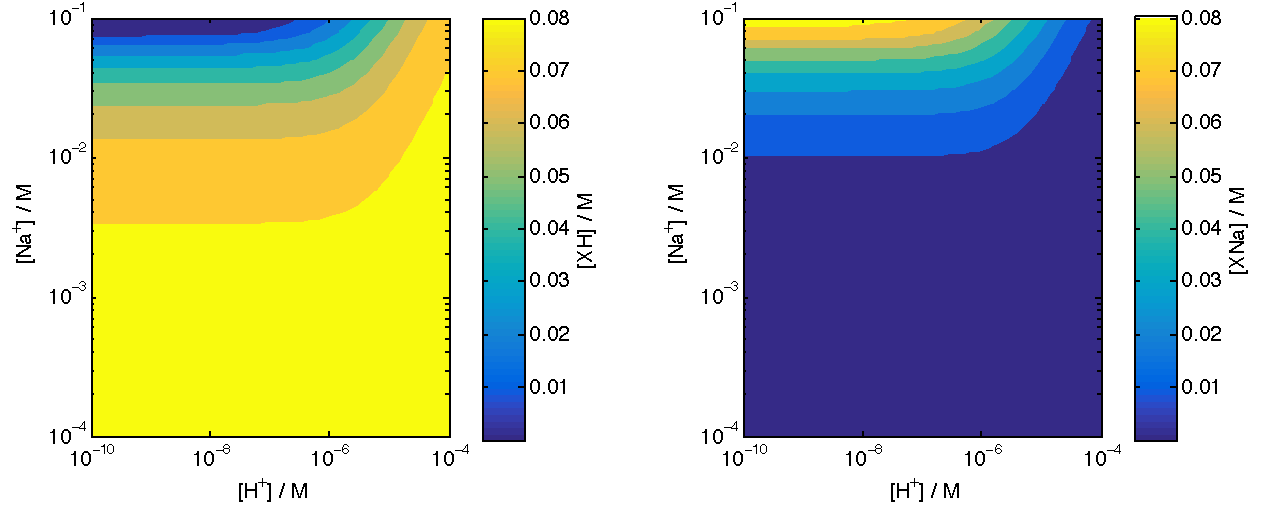
\includegraphics[width=0.9\textwidth]{sweep.pdf}
    \caption{The effect of pH and salinity on chemistry of ion-exchange surface.}
    \label{fig:my_label}
\end{figure}

This functionality makes the solver especially well suited for transport calculations where the chemistry of every cell in the mesh must be solved. If the user is so inclined, temperature, reaction constants, and surface geometry parameters can all accept vector inputs.

\section{Post processing}

In solving the chemical system \verb|initState| populates \verb|state| with the determined values for total element concentration and species concentrations. Depending on the chemical system \verb|state| may also contain linear combination concentrations, gas phase pressures, solid phase saturation indices, and surface activity coefficient multipliers. MATCH provides additional tools to further gleam information from the state variables, including additional calculations.

\subsection{Accessing information in \texttt{state}}
The structure \verb|state| contains an abundance of information. To access the variables MRST provides the \verb|getProps| tool. Given the \verb|ChemicalModel| object and the \verb|state| structure any solved variable can be easily extracted. 

Inside of the \verb|ChemicalModel| object are lists of variable names, as well as the field in which they live within \verb|state|. The position of the variable name within the list corresponds to the column that variable occupies within the appropriate field. Using this information, \verb|getProps| can retrieve the value of any variable from state. Take the simple example
\begin{lstlisting}
elementNames = {'O', 'H', 'Na*', 'Cl*'};

speciesNames = {'H+*', 'OH-', 'Na+', 'Cl-', 'NaCl', 'H2O*'};

reactions = {'H2O  = H+  + OH- ', 10^-14*mol/litre, ...
             'NaCl = Na+ + Cl-',  10^1*mol/litre};

chem = ChemicalModel(elementNames, speciesNames, reactions);

Na  = 1*milli*mol/litre;
Cl  = 1*milli*mol/litre;
H2O = 1*mol/litre;
H   = 1e-7*mol/litre;

inputs = [Na, Cl, H, H2O];

state = chem.initState(inputs);
\end{lstlisting}
The user can now retrieve the value of any of the un/knowns from \verb|state| without any knowledge of the variable's location within \verb|state| using the variable names as they are defined in the chemical model. For instance to determine the concentration of hydroxide

\begin{lstlisting}
>>chem.getProps(state, 'OH-')

ans =

   1.0739e-04
\end{lstlisting}
Remember that all variables are stored in SI units, and so concentrations are mol/m$^3$. To retrieve multiple variables at once use the function \verb|getProps|.

\begin{lstlisting}
[OH_minus, H_tot] =chem.getProps(state, 'OH-', 'H')
\end{lstlisting}
The above code returns the concentration of hydroxide and the total concentration of hydrogen in the system. Similarly, lists of names can used to pull multiple variables from \verb|state|. For instance the concentration of all species can be grabbed simultaneously:

\begin{lstlisting}
speciesConc = cell(1, numel(chem.speciesNames));

[speciesConc{:}] =chem.getProps(state, chem.speciesNames{:});
\end{lstlisting}

The ChemicalModel object contains a number of useful lists by default including
\begin{description}
        \item[\texttt{elementNames}] names of elements (basis components)
        \item[\texttt{speciesNames}] names of species
        \item[\texttt{solidNames}] names of solid phases
        \item[\texttt{gasNames}] names of gas phases
        \item[\texttt{surfaceActivityCoefficientNames}] names of surface potential multipliers
        \item[\texttt{combinationNames}] names of combination components
\end{description}
Additionally there are lists of the log names of each variable (i.e. \verb|logElementNames|). For instance the $\log_e$ of the hydroxide concentration can be retrieved by asking \verb|getProps| for \mcode{'logOH-'}. There is no log form of the entries of \verb|combinationNames| as the value of combination components can be negative. 

The user can also ask for the contents of an entire field by asking \verb|getProps| for the field name (i.e. \mcode{chem.getProp(state, 'elements')} to get all element concentrations).

\subsection{Additional calculations}

MATCH includes several tools to aid in processing the results of the chemical system solver. These include

\begin{description}
        \item[\texttt{computeActivities}] computes the activity of aqueous species storing the results in \verb|state.activities|.
        \item[\texttt{computeChargeBalance}] computes the charge balance of the system, storing the results in \verb|state.chargeBalance|.
        \item[\texttt{computeSurfacePotentials}] computes the electric potential of each plane of each electrostatic surface group, storing the results in \verb|state.surfacePotentials|
        \item[\texttt{computeSurfaceCharges}] computes the charge of each plane of each electrostatic surface group, storing the results in \verb|state.surfaceCharges|
        \item[\texttt{computeAqueousConcentrations}] computes the aqueous concentration of each element, excluding gas, solid, and surface concentrations, the results are stored in \verb|state.aqueousConcentrations|
        \item[\texttt{computeSurfaceConcentrations}] computes the surface concentration of each element \verb|state.surfaceConcentrations|
        \item[\texttt{changeUnits}] changes the units of any field of \verb|state|
\end{description}

\subsubsection{computeActivities}

In MATCH the activity of aqueous species is calculated by the extended Davies equation. The activity of each aqueous species can be retrieved once the chemical solver has populated \verb|state| by

\begin{lstlisting}
[state, chem] = chem.computeActivities(state);
\end{lstlisting}
The above code returns \verb|state| with the additional field \verb|activities|. The \verb|ChemicalModel| object is also returned with the additional field \verb|activityNames|. The activity of aqueous species can be retrieved from \verb|state| by asking \verb|getProps| for the species name prepended with 'a' (i.e. \mcode{chem.getProp(state, 'aH+')} for the activity of \ce{H+}). The activity of surface species is not added to \verb|state.activities|. The activity of all aqueous species can be retrieved by \mcode{chem.getProps(state,'activities')}. The activity of electrons \ce{e-} is also included, but \ce{e-} does not contribute to the ionic strength of the solution.

\subsubsection{computeChargeBalance}

The charge balance of the aqueous system can be retrieved once the chemical solver has populated \verb|state| by

\begin{lstlisting}
[state, chem] = chem.computeChargeBalance(state);
\end{lstlisting}

The above code returns \verb|state| with the additional field \verb|chargeBalance|. The \verb|ChemicalModel| object is also returned and made aware of the new field in \verb|state|. The charge balance of the system can be retrieved from \verb|state| by asking \verb|getProps| for the \mcode{'chargeBalance'} (i.e. \mcode{chem.getProp(state, 'chargeBalance')}). The charge of electrons \ce{e-} does not contribute to charge balance. 

\subsubsection{computeSurfacePotentials}

In MATCH the potential of each electrostatic surface group and layer therein can be retrieved once the chemical solver has populated \verb|state| by

\begin{lstlisting}
[state, chem] = chem.computeSurfacePotentials(state);
\end{lstlisting}
The above code returns \verb|state| with the additional field \verb|surfacePotentials|. The \verb|ChemicalModel| object is also returned with the additional field \verb|surfacePotentialNames|. The potential of each surface and layer can be retrieved from \verb|state| by asking \verb|getProps| for the surface name, as determined by the \verb|groups| key, or by the surface functional group name, appended by \mcode{'_Psi_#'} where '\#' is the layer of the surface. \mcode{'Psi'} is used as the surface potential is often denoted as $\Psi$ in the literature. As an example, to retrieve the potential of a triple layer surface \ce{SiO}

\begin{lstlisting}
chem.getProps(state, '>SiO_Psi_0', '>SiO_Psi_1', '>SiO_Psi_2');
\end{lstlisting}
where \mcode{'>SiO_Psi_0'} is the potential of the mineral surface, \mcode{'>SiO_Psi_1'} is the potential of the inner Helmholtz plane and \mcode{'>SiO_Psi_2'} is the potential of the outer Helmholtz plane. If the constant capacitance model was used, only one surface potential exists and can be retrieved by \mcode{chem.getProps(state, '>SiO_Psi')}, where no number is appended. The electric potential of surfaces is given in volts, the SI unit. The potential of Langmuir and ion exchange surfaces is not computed. If a surface was defined using the 'groups' key inside of \verb|surfaces| then the group name would be used. For example, as above, several oxide surfaces were grouped in the \mcode{'Goe'} (goethite) surface. To retrieve the value of the mineral surface potential the user would ask for \mcode{chem.getProps(state, 'Goe_Psi_0')}.

\subsubsection{computeSurfaceCharges}

In MATCH the charge density of each surface and layer therein can be retrieved once the chemical solver has populated \verb|state| by

\begin{lstlisting}
[state, chem] = chem.computeSurfaceCharges(state);
\end{lstlisting}
The above code returns \verb|state| with the additional field \verb|surfaceCharges|. The \verb|ChemicalModel| object is also returned with the additional field \verb|surfaceChargeNames|. The charge density of each surface and layer can be retrieved from \verb|state| by asking \verb|getProp| for the surface name, as determined by the \verb|groups| key, or by the surface functional group name, appended by \mcode{'_sig_#'} where '\#' is the layer of the surface. \mcode{sig} is used as the surface charge density is often denoted as $\sigma$ in the literature. As an example, to retrieve the charges of a triple layer surface \ce{SiO}

\begin{lstlisting}
chem.getProps(state, '>SiO_sig_0', '>SiO_sig_1', '>SiO_sig_2');
\end{lstlisting}
where \mcode{'>SiO_sig_0'} is the charge density of the mineral surface, \mcode{'>SiO_sig_1'} is the charge density of the inner Helmholtz plane and \mcode{'>SiO_sig_2'} is the charge density of the outer Helmholtz plane. The surface charge density is given in C/m$^2$, the SI unit. If the Langmuir or constant capacitance model was used, only one surface charge density exists and can be retrieved by \mcode{chem.getProps(state, '>SiO_sig')}, where no number is appended. The surface charge density of all surface \emph{except} ion exchange surfaces can be retrieved using \verb|computeSurfaceCharges|. If a surface was defined using the 'groups' key inside of \verb|surfaces| then the group name would be used. For example, as above, several oxide surfaces were grouped in the \mcode{'Goe'} (goethite) surface. To retrieve the value of the mineral surface charge density the user would ask for \mcode{chem.getProps(state, 'Goe_sig_0')}.

\subsubsection{computeAqueousConcentrations}

In MATCH the total aqueous concentration of an element can be retrieved once the chemical solver has populated \verb|state| by

\begin{lstlisting}
[state, chem] = chem.computeAqueousConcentrations(state);
\end{lstlisting}
The above code returns \verb|state| with the additional field \verb|aqueousConcentrations|. The \verb|ChemicalModel| object is also returned with the additional field \verb|aqueousConcentrationNames|. The total aqueous concentration of an element can be retrieved from \verb|state| by asking \verb|getProp| for the element name appended by \mcode{'(aq)'} (i.e. \mcode{chem.getProp(state, 'H(aq)')} for the total aqueous concentration of hydrogen). The total aqueous concentration of all elements can be retrieved by \mcode{chem.getProp(state,'aqueousConcentrations')}. The total aqueous concentration of surface functional groups is not added to \verb|aqueousConcentrations|.

\subsubsection{computeSurfaceConcentrations}

In MATCH the total surface concentration of an element can be retrieved once the chemical solver has populated \verb|state| by

\begin{lstlisting}
[state, chem] = chem.computeSurfaceConcentrations(state);
\end{lstlisting}
The above code returns \verb|state| with the additional field \verb|surfaceConcentrations|. The \verb|ChemicalModel| object is also returned with the additional field \verb|surfaceConcentrationNames|. The total surface concentration of an element can be retrieved from \verb|state| by asking \verb|getProp| for the element name appended by \mcode{'(surf)'} (i.e. \mcode{chem.getProp(state, 'H(surf)')} for the total surface concentration of hydrogen). The total surface concentration of all elements can be retrieved by \mcode{chem.getProp(state,'surfaceConcentrations')}. The total surface concentration of surface functional groups is not added to \verb|surfaceConcentrations| as this would be equivalent to the total concentration, as surface functional groups do not reside in the liquid. 

\subsubsection{changeUnits}
\verb|changeUnits| is not a function inside of the \verb|ChemicalModel| object, and so should be called with the object name:

\begin{lstlisting}
state = changeUnits(state, fields, unit_conv);
\end{lstlisting}
where \verb|fields| is a cell array of field names that are inside of \verb|state| and \verb|unit_conv| is a scalar or vector of the unit conversion. Take for instance the conversion of all species concentrations from the SI unit of mol/m$^3$ to the more common mol/litre

\begin{lstlisting}
state = changeUnits(state, {'species'}, mol/litre);
\end{lstlisting}

If you want to do the same conversion to multiple fields, \verb|unit_conv| can stay as a scalar

\begin{lstlisting}
state = changeUnits(state, {'species', 'elements', 'activities'}, mol/litre);
\end{lstlisting}
Or each field can have different units

\begin{lstlisting}
state = changeUnits(state, {'species', 'elements', 'activities'}, [mol/litre, milli*mol/litre, kilo*mol/(nano*meter)^3]);
\end{lstlisting}

\section{Transport simulations}

MATCH has the ability to simulate the advection-reaction equation on arbitrary domains using a fully implicit upwind finite volume scheme. The procedure for such a simulation follows the steps
\begin{enumerate}
    \item define a domain geometry
    \item define fluid and rock properties
    \item define a chemical system
    \item solve the chemical system for the conditions in the domain
    \item specify boundary conditions, wells, and source terms
    \item define a time stepping schedule
    \item run the simulation
\end{enumerate}

The MRST guidebook has a wealth of knowledge for the grid generation \cite{lie2014}, and several examples are provided for reference. We will use a simple system as an example to introduce the above concepts

\begin{lstlisting}
close all;
clear;

mrstModule add ad-core ad-props ad-blackoil geochemistry mrst-gui

%% Define the grid
G = cartGrid([100, 1, 1], [1, 1, 1]);
G = computeGeometry(G);
\end{lstlisting}

Here we loaded the necessary modules for the transport simulation and have defined a 1D domain of size 1m$\times$1m$\times$1m, and a discretization of 100$\times$1$\times$1 cells. 

We must now define a fluid and rock so that the transport properties of the porous medium can be calculated

\begin{lstlisting}
%% Define the rock
rock.perm = 1*darcy*ones(G.cells.num, 1);
rock.poro = 0.5*ones(G.cells.num, 1);

%% Define the fluid
pRef = 0*barsa;
fluid = initSimpleADIFluid('phases', 'W', 'mu', 1*centi*poise, 'rho', ...
                           1000*kilogram/meter^3, 'c', 1e-10, 'cR', 4e-10, ...
                           'pRef', pRef);
\end{lstlisting}

Here we have defined a rock object with a permeability of 1 Darcy and porosity of 0.5 as well as a single liquid phase, water. For more information on the fluid and rock objects see the MRST book \cite{lie2014}.

In this example we will simulate the injection of a fluid with distinct composition into a resovoir at equilibrium with a fluid of a different composition. We define the system chemical system as before, but solve for two composition, one for in initial fluid, and one for the injected. 

\begin{lstlisting}
%% Define the chemistry
elements = {'O', 'H', 'Na*','Cl*'};

species = {'H+*', 'OH-', 'Na+', 'H2O*', 'NaCl','Cl-'};

reactions ={'H2O  = H+  + OH- ',      10^-14*mol/litre, ... 
            'NaCl = Na+ + Cl-',       10^1*mol/litre};

% instantiate chemical model
chemModel = ChemicalModel(elements, species, reactions);

% initial chemistry
Nai = 1e-3;
Cli = Nai;
Hi = 1e-7;
H2Oi = 1;

initial = [Nai Cli Hi H2Oi]*mol/litre;

[initChemState, initReport]= chemModel.initState( repmat(initial, G.cells.num, 1), 'charge', 'Cl');

% injected chemistry
Naf = 1e-3;
Clf = Naf;
Hf = 1e-10;
H2Of = 1;

injected = [Naf Clf Hf H2Of]*mol/litre;

[injChemState, injreport]= chemModel.initState(injected, 'charge', 'Cl');
\end{lstlisting}

The transport equation evolves the total element concentration. The flow field is calculated by solving the pressure field. Thus pressure must be added to the \mcode{state} structure.
\begin{lstlisting}
initChemState.pressure          = pRef*ones(G.cells.num, 1);
\end{lstlisting}

The transport model object is instantiated using the \mcode{ChemicalTransportModel} command

\begin{lstlisting}
model = ChemicalTransportModel(G, rock, fluid, chemModel);
\end{lstlisting}

and accepts the domain geoemtry, rock, fluid and chemical model objects. Next the boundary conditions must be specified. In this example we will be injecting the new fluid into the first cell via a Neumann boundary condition on the left hand side. On the right hande side of the domain we specify a Dirchlet boundary condition with a reference pressure of 0.

\begin{lstlisting}
src                	= [];
src               	= addSource(src, 1, 1*meter^3/day, 'sat', 1);
src.elements        = injChemState.elements(end,:);
src.logElements     = injChemState.logElements(end,:);

bc                  = [];
bc                  = pside(bc, 'east', 0*barsa, 'sat', 1);
bc.elements         = initChemState.elements(end,:);        % (will not used if outflow)
bc.logElements      = initChemState.logElements(end,:);  % (will not used if outflow)
\end{lstlisting}

Note that the element concentrations will only be used if the boundary condition is an inflow. If the chemical system involves surface species, their concentration should not be added to the boundary condition. The transport model object contains a matrix multiplier called \mcode{fluidMat} which can be used to remove their contribution. See the example file \mcode{surfaceSystemTransport.m} for a demonstration. 

Next an injection schedule must be specified

\begin{lstlisting}
%% Define the schedule
schedule.step.val = [0.01*day*ones(5, 1); 0.1*day*ones(5,1); 1*day*ones(5, 1); 5*day*ones(10, 1)];
schedule.step.control = ones(numel(schedule.step.val), 1);
schedule.control = struct('bc', bc, 'src', src, 'W', []);
\end{lstlisting}

Here we take five steps of 0.01 days, 5 steps of 0.1 days, 5 steps of 1 day and then 10 steps of 5 days. The transport solver will have an easier time converging is the time stepping is ramped up in such a way. 

Finally, the transport simulation can be run. 

\begin{lstlisting}
[wellsols, states, scheduleReport] = simulateScheduleAD(initChemState, model, schedule);
\end{lstlisting}

The function will return a cell array of \mcode{state} structures corresponding to every time state in the system, as well as a solver report for each of the steps. In the case that a well is also specified the well solutions will be returned.

The results of the simulation can be visualized with the \mcode{plotToolbar} function.

The simulation progress can be visualized by toggling the two options \mcode{model.plotIter} and \mcode{model.plotFinal}. Both options are set to \mcode{false} by default. With these options the solver will plot the elements and species distribution in the domain for each iteration of the newton solver, and at each time step once the solver has converged. 

\section{Equations of the chemical system}
The chemical system is determined by the following equation
\begin{itemize}
    \item conservation of mass for each basis component/element
    \item laws of mass action relating species concentrations through chemical reactions
    \item equilibrium between gas-liquid and solid-liquid phases
    \item aqueous charge balance [optional]
    \item surface charge balance [depending on surface chemistry model]
    \item transport law [optional]
\end{itemize}

Below we will formally introduce these equations. For convenience the variables and nomenclature are presented in Table \ref{table:variables}.

\begin{table}[H]
\centering
\caption{Nomenclature of variables used in equations.}
\label{table:variables}
\begin{tabular}{l|l|l|l}
\toprule
variable        & unit                      & index                     & description                           \\ \midrule
$N_i$           & mol/m$^3$                 & $i = \{1 \ldots n_b\}$    & total concentration of element $i$                        \\
$c_j$           & mol/m$^3$  or [-]         & $j = \{1 \ldots n_c\}$    & concentration or mole fraction of species $j$                      \\
$\gamma_j$      & -                         & -                         & activity coefficient of species $j$                      \\
$\alpha_{i,j}$  &    -                      & -                         & mass contribution of element $i$ to species $j$ \\
$z_j$           &    -                      & -                         & charge of species $j$ \\
$g_k$           & Pa                        & $k = \{1 \ldots n_g\}$    & partial pressure of gas phase $k$                         \\
$K_l$           & dependent on $l$          & $l = \{1 \ldots n_r\}$    & equilibrium constant of reaction $l$, excluding solid phase reactions                      \\
$\beta_{j,l}$   & -                         & -                         & stoichiometric coefficient of species $j$ in reaction $l$\\
$S_m$           & -                         & $m = \{1 \ldots n_s\}$    & saturation index of solid phase $m$                      \\
$Q_m$           & dependent on $m$          & -                         & equilibrium constant of solid phase reaction $m$         \\
$\eta_{j,m}$    & -                         & -                         & stoichiometric coefficient of species $j$ in solid phase reaction $m$\\
$S_o$           & m$^2$/kg                  & $o = \{1 \ldots n_e\}$    & specific surface area of electrostatic surface $o$        \\
$a_o$           & kg/m$^3$                  & -                         & slurry density of electrostatic surface $o$        \\
$C_{o,q}$       & F/m$^2$                   & $q = \{1 \ldots n_l\}$    & capacitance of layer $q$ of electrostatic surface $o$        \\
$\sigma_{o,p}$  & C/m$^2$                   & $p = \{1 \ldots n_p\}$    & charge density of plane $p$ of electrostatic surface $o$        \\
$\Psi_{o,p}$    & V                         & -                         & electric potential of plane $p$ of electrostatic surface $o$        \\
$\zeta_{j,o,p}$ & -                         & -                         & charge contribution of species $j$ to plane $p$ of electrostatic surface $o$ \\
$L_{u}$         & mol/m$^3$                 & $u = \{1 \ldots n_w\}$    & concentration of linear combination $u$ \\
$\xi{j,u}$      & -                         & -                         & mass contribution of species $j$ to linear combination $u$ \\
$U_i$           & mol/(m$^2$s)              & -                         & flux of element $i$\\
$F_i$           & mol/(m$^3$s)              & -                         & source of element $i$\\
$\vec{U}$       & m$^3$/(m$^2$s)            & -                         & volumetric flow rate of element $i$\\
\bottomrule
\end{tabular}
\end{table}

And the parameters used within MATCH are presented in Table \ref{table:params}

\begin{table}[H]
\centering
\caption{Parameters and constants used in MATCH.}
\label{table:params}
\begin{tabular}{l|l|l|l}
parameter       & value                      & units                     & description                           \\ \toprule
$A_n$           & $6.022140857 \times 10^{23}$           & \#/mol                   & Avagadro's number                      \\
$e_o$           & $8.8854187817 \times 10^{-12}$        & F/m                      & permitivity of free space                      \\
$e_w$           & -                          & -                        & dielectric constant of water                      \\
$F$             & 96485.33289                          & C/mol                        & Faraday's constant                      \\
$R$             & 8.3144598                          & J/(K mol)                        & ideal gas constant                      \\
$T$             & -                          & K                       & temperature                      \\
$I$             & -                          & mol/m$^3$                       & ionic strength of solution                      \\
\bottomrule
\end{tabular}
\end{table}


\subsection{Conservation of mass}
In the absence of sink and source terms the conservation of total element concentration in the system is constant
\begin{align}
    N_i = \sum_{j=1}^{n_c} \alpha_{i,j} c_j,
\end{align}
where $N_i$ is the concentration of element $i$, $n_c$ is the number of total number of species, $\alpha_{i,j}$ is the mass contribution of element $i$ to species $j$, and  $c_j$ is the concentration of species $j$. The variables $c$ and $N$ includes surface functional groups and surface bound species. Note that the mass of elements in the gas a solid phase do not contribute to the mass constraint in the model formulation. In the conservation of mass equations, all species concentrations $c_j$ are in units of moles/m$^3$ including surface species. 

\subsection{Laws of mass action}
The laws of mass action determine the equilibrium distribution of species under the constrain of local chemical equilibrium

\begin{align}
K_l = \prod_{j=1}^{n_c} \left(\gamma_j c_j\right)^{\beta_{j,l}}.
\end{align}
Where $K_l$ is the equilibrium constant of reaction $l$, $\gamma_j$ is the activity coefficient of species $j$, and $\beta_{j,l}$ is the stoichiometric coefficient of species $j$ in reaction $l$.  Note that $\beta$ can be positive, negative, or zero if the species is a reactant, a product, or absent respectively. Note that $K$ does not include solid phase reactions, but does include gas phase reactions, surface reactions, and aqueous reactions. For the laws of mass actions, if species $j$ resides on the surface $c_j$ is the mole fraction of the surface species as defined by model 3 in \citet{wang2013}{}. This is the case for all the surface models used in MATCH.

\subsection{Activity of aqueous species}
The activity of aqueous species $\gamma_j$ is determined by the extended Davies equation

\begin{align}
    \log_{10}\left(\gamma_j\right) = A z_j^2\left(\dfrac{I^{1/2}}{1+I^{1/2}} - 0.3I\right),
\end{align}
where $z_j$ is the charge of species $j$, and $I$ is the ionic strength of the bulk solution. The parameter $A$ being determined by

\begin{align}
    A = 1.82\times10^6 \left(e_wT\right)^{-3/2}.
\end{align}
where $e_w$ is the relative permeability of water, and $T$ is the temperature of the bulk solution \cite{Davies1962}{}. The dielectric constant of water is determined by the polynomial function

\begin{align}
    e_w = 87.740 - 0.4008(T-273.15) + 9.398\times10^{-4}(T-273.15)^2 - 1.410\times10^{-6}(T-273.15)^3
\end{align}
as presented by \citet{malmberg1956dielectric}{}.
The ionic strength of the solution is calculated by

\begin{align}
    I = \dfrac{1}{2}\sum_{j=1}^{n_c} z_j c_j \delta_j
\end{align}
where in this case $\delta$ removes the contribution of charge from surface species, and the electron \ce{e-}.

\begin{align}
\delta_j = \begin{cases}
0, \quad\text{if species $j$ on a surface or is \ce{e-}},\\
1, \quad\text{otherwise}.
\end{cases}
\end{align}

\subsection{Activity of surface species}
The activity of surface species depends on the surface chemistry model that is employed. The activity of species associated with a Langmuir type surface is 1.

\subsubsection{Ion exchange surfaces}
The activity of species associated with ion exchange type surfaces is determined by their active fraction consistent with the Gaines-Thomas convention \cite{gaines1953}{}.

\subsubsection{Electrostatic surface}
The activity of species associated with an electrostatic surface (such as the triple layer and constant capacitance models) are determined by the potential and charge of the planes which the species occupy, 

\begin{align}
    \gamma_j = \exp\left(\dfrac{F\sum_{p=1}^{n_p}\zeta_{j,o,p}\Psi_{o,p}}{RT}\right)\label{eq:surfAct}
\end{align}
where $F$ is Faraday's constant, $\zeta_{j,o,p}$ is the charge contribution of species $j$ to plane $p$ of electrostatic surface $o$, $\Psi_{o,p}$, is the electric potential of the $p^\text{th}$ plane of the $o^\text{th}$ electrostatic surface and $R$ is the ideal gas constant \cite{Hiemstra1989a}{}. Note that a surface species can be associated with multiple surface functional groups, but only one electrostatic surface

\subsection{Electrostatics of the surface}

For a full description and comparison of different surface chemistry models consult \citet{westall1980}{}, which is the text that the constitutive relationships shown here are pulled from. 

\subsubsection{Constant Capacitance model}
Only one layer exists in the constant capacitance model, the mineral surface. The charge of the mineral surface, $\sigma$, is calculated as the linear combination of charged species which reside on the surface

\begin{align}
    \sigma_{o,p=1} = \dfrac{F}{S_o a_o}\sum_{j=1}^{n_c}c_j\zeta_{j,o,p=1}
\end{align}
where $\sigma_{o,p=1}$ is the charge density of the mineral surface of the $o^\text{th}$ electrostatic surface (which is a constant capacitance surface), and $S_o$ and $a_o$ are the specific surface area and slurry density of electrostatic surface $o$. Note the charge contribution of a species to an electrostatic surface on which it does not reside will be zero.

The constant capacitance model simulates the mineral-liquid interface as a capacitor. The potential is therefore determined by the capacitance density of the interface

\begin{align}
    \Psi_{o,p=1} = \dfrac{\sigma_{o,p=1}}{C_{o,q=1}}
\end{align}
where $C_{o,q=1}$ is the capacitance density of the $o^\text{th}$ electrostatic surface, being of type constant capacitance. And where $q$ is the index of the layer, the constant capacitance model only having one.  

Note that charge neutrality is not enforced for constant capacitance surfaces. 
\subsubsection{Triple layer model}

The triple layer model approximates the mineral-liquid interface as three capacitors in series. The first two, starting from the mineral surface have a constant capacitance density, the outer most layer has a variable capacitance density as determined by the properties of the bulk solution according to the Grahame equation. Just as in the constant capacitance model the charge of a plane is the linear summation of charged species that reside of the plane. While the charge density of the outer layer is determined by the Grahme equation

\begin{align}
\sigma_{o,p} &= \dfrac{F}{S_o a_o}\sum_{j=1}^{n_c}c_j\zeta_{j,p} - (8\times10^3 R T I e_o e_w)^{1/2}\sinh\left(\dfrac{F\Psi_{o,p}}{2RT}\right)\delta_m\label{eq:charge}
\end{align}
where 

\begin{align}
\delta_m = \begin{cases}
1, \quad\text{if m=3},\\
0, \quad\text{otherwise}.
\end{cases}
\end{align}

The charge-potential relationship for the triple layer surface is then determined by
\begin{align}
\sigma_{o,p=1}  &= C_{o,q=1}\left(\Psi_{o,p=1} -\Psi_{o,p=2}\right)\label{eq:pot1}\\
\sigma_{o,p=3}  &= C_{o,q=2}\left(\Psi_{o,p=3} -\Psi_{o,p=2}\right)\label{eq:pot2}
\end{align}
Finally the triple layer surface must be charge neutral

\begin{align}
    0 = \sum_{i=1}^{n_p} \sigma_{i,p}.\label{eq:neutral}
\end{align}

\subsection{Equilibrium with solid phases}

Strictly speaking, equilibrium with solid phases is not enforced, rather the saturation index is. The saturation index, SI, is the ratio of the ion association product and the equilibrium constant of the precipitation reaction
\begin{align}
\text{SI}_m = \dfrac{\prod_{j=1}^{n_c} \left(\gamma_j c_j\right)^{\eta_{j,m}}}{Q_m},
\end{align}
where $\text{SI}_m$ is the saturation index of solid phase $m$, $\eta_{j,m}$ is the stoichiometric coefficient of species $j$ in solid phase reaction $m$, and $Q_m$ is the equilibrium constant of solid phase reaction $m$. When $\text{SI}_m<1$ the solution is undersaturated with respect to the solid phase, when $\text{SI}=1$ the solution is saturated and when $\text{SI}>1$ the solution is supersaturated. Note that some chemical solvers use the $\log_{10}$ of the above ratio. 

\subsection{Linear combinations}
MATCH allows the user to define custom linear combination components $L$

\begin{align}
    \hat{L}_u = \sum_{j=1}^{n_c} \xi_{j,u} c_j, % + \sum_{i=1}^{n_b} \nu_{i,u} N_i
\end{align}
where $L_u$ is the concentration of linear combination $u$, $\xi_{j,u}$ is the stoichiometric contribution of species $j$ to linear combination $u$. MATCH does not allow solid and gas phases to enter into linear combinations.

\subsection{Charge balance}
The user may choose whether to enforce charge balance. Charge balance only considers the charge of aqueous species, disregarding the contribution of surface species and the electron \ce{e-}. There should be no charged species in the gas and solid phases. The sum of all positive and negative charges should be equal when charge balance is enforced

\begin{align}
    0 = \sum_{j=1}^{n_c} z_j c_j \delta_j
\end{align}
where $\delta$ turns off the contribution of \ce{e-}, and surface species
\begin{align}
\delta_j = \begin{cases}
0, \quad\text{if species $j$ is on a surface or is \ce{e-}},\\
1, \quad\text{otherwise}.
\end{cases}
\end{align}

It is possible that charge balance can not be achieved with the mass constraints specified by the user, as the addition of the charge balance equation makes the system over determined. Therefore to achieve charge balance and a well posed problem we relax the user supplied constraint on the charge variation component so that it is an unknown. This ensure there are an equal number of unknowns and equations.

\subsection{Transport}

The governing equations for the transport of chemical elements can be written
\begin{equation}
  \label{eq:transgen}
  \fracpar{N_i}{t} + \dive \vec{U_i} = F_i(N)
\end{equation}
where the flux $U_i$ is defined by
\begin{align}
    \vec{U_i} = \sum_{j=1}^{n_c} \alpha_{i,j} c_j \vec{U} \delta_j
\end{align}
where $\delta$ here is defined as
\begin{align}
  \delta_j =
  \begin{cases}
    1 &\text{ if the component $j$ is a dissolved species,}\\
    0 &\text{ if the component $j$ is a solid, gas, or surface species}
  \end{cases}
\end{align}

The determination of the flow field $\vec{U}$ depends on the physical system. For a detailed discussion of these physics see the MRST book \cite{lie2014}. 
The transport law is solved fully implicitly, with a upwind difference scheme in space. 


\subsection{a priori bounds on variables}

The structure of the chemical system allows for natural a priori bounds on variables of the nonlinear system. 
The total concentration of basis components in the system is bound by 

\begin{align}
    \texttt{realmin} \leq N_i \leq 300,000 \text{\;mol/m$^3$}.
\end{align}
The concentration of water in water typically being around 55,000 mol/m$^3$, which corresponds to a total hydrogen concentration of 110,000 mol/m$^3$. It is unlikely that any other species would appreciablly raise the total concentration of elements close to this upper bound.

The maximum concentration of a species can obtain is the proportional summation of all elements/basis components which comprise that species
\begin{align}
   \hat{c}_j = \sum_{i=1}^{n_b} \alpha_{i,j}^{-1}N_i 
\end{align}
where $\hat{c}_j$ is the maximum value of $c_j$. Entries of $\alpha$ that are zero are removed prior to the operation. The species concentration is bounded by

\begin{align}
    \texttt{realmin} \leq c_j \leq  \hat{c}_j
\end{align}
 Similarly, the maximum value of linear combinations is linear summation of the elements and species that make up the components

\begin{align}
    \hat{L}_u =\sum_{j=1}^{n_c} \hat{c}_j|\xi_{j,u}|, %+ \sum_{i=1}^{n_b}|\nu_{q,j}|N_i,
\end{align}
where $L$ is bounded by

\begin{align}
    -|\hat{L}_{u}| \leq L_{u} \leq |\hat{L}_{u}|.
\end{align}

For the triple layer model the maximum potential of surface layers is calculated by first determining the maximum charge of the mineral surface

\begin{align}
    \hat{\sigma}_{o,p=1} &= \max_{j,p}(|\zeta_{j,o,p}|)\dfrac{F}{S_o a_o}\sum_{i=1}^{n_b} N_i \delta_i.
\end{align}
where $\hat{\sigma}_{o,p}$ is the maximum value of $\sigma_{o,p}$ and $\delta_i=1$ if element $i$ is a functional group associated with electrostatic surface $o$
and $\delta_i=0$ otherwise. The maximum values of potential are obtained from a simplification of \eqref{eq:charge}-\eqref{eq:neutral}

\begin{align}
    \hat{\sigma}_{o,p=3} &= \hat{\sigma}_{o,p=1},\\
    \hat{\Psi}_{o,p=3} &= \dfrac{2RT}{F}\sinh^{-1}\left(\dfrac{-\hat{\sigma}_{o,p=3}}{(8\times10^3 R T I e_o e_w)^{1/2}}\right),\\
    \hat{\Psi}_{o,p=2} &= \hat{\Psi}_{o,p=3}\\ 
    \hat{\Psi}_{o,p=1} &= \hat{\Psi}_{o,p=3}.
\end{align}
The electric potential is bounded by 

\begin{align}
    -|\hat{\Psi}_{o,p}| \leq \Psi_{o,p} \leq |\hat{\Psi}_{o,p}|.
\end{align}

\subsection{log transformation of variables}

The numerical solution of chemical systems is made difficult by the large condition number of the nonlinear system. To mediate this problem MATCH performs a $\log_e$ transformation on all variables \emph{except} CVC, and $L$. The unknowns of the chemical system are then the $\log_e$ of concentrations, potential, saturation indices and partial pressures. The transformation reduces the reaction equations to a set of linear equations, however, the linear combination and mass constraint equations are now nonlinear, though slightly (we think) better behaved than the original nonlinearity in the reaction equations. Another important point is that the $\log_e$ transformation reduces the surface activity multiplier, as seen in \eqref{eq:surfAct}, from exponential to linear. The original values are retrieved by taking the exponential of all transformed variables after the solver has converged. 

We hope to present the full mathematical analysis of the $\log_e$ system in the coming months, along with numerical tests. 
\section{Examples}
Several example scripts are provided in the \verb|examples| folder of the repository. All files include examples of defining the chemical system, choosing components as inputs, creating input vectors and passing those inputs to the solver. 
\begin{description}
        \item[\texttt{simpleSystem.m}] Calculates aqueous speciation of \ce{H2O} and \ce{NaCl} under varying pH conditions.
        \item[\texttt{alkalinity.m}] Carbonate speciation with alkalinity as an input, using linear combination.
        \item[\texttt{constantCapacitance.m}] Boron adsorption onto soil using the constant capacitance model.
        \item[\texttt{tripleLayerModel.m}] Silica surface speciation using the triple layer model.
        \item[\texttt{ionExchange.m}] Competition of protons and sodium for an ion exchange site.
        \item[\texttt{phases.m}] Carbonate system with precipitation and gas phase equilibrium.
        \item[\texttt{redoxChemsitry.m}] Speciation of nitrogen between oxidation states as a function of pe and pH.
        \item[\texttt{simpleSystemTransport.m}] Transport of the \ce{H2O} and \ce{NaCl} system on a 2D domain with source terms.
        \item[\texttt{surfaceSystemTransport.m}] Transport on a 1D domain of a system with sorption.
        \item[\texttt{solidSystemTransport.m}] Transport on a 1D domain of a system with solid phase.
\end{description}

\section{Comparison to PHREEQC}

Here we present several examples which test the functionality within MATCH by a comparison to solutions obtained using the USGS maintained program PHREEQC \cite{parkhurst1999}{}.

\subsection{Aqueous speciation}
Here we explore the chemical system

\begin{align}
    \ce{H2O} &= \ce{H+} + \ce{OH-}\\
    \ce{NaOH}&= \ce{Na+} + \ce{OH-}\\
    \ce{HCl} &= \ce{H+} + \ce{Cl-}\\
    \ce{Ca^{+2}} + \ce{H2O} &=\ce{CaOH+} + \ce{H+}
\end{align}
including charge balance. We provide the system with inputs
\begin{align}
\Sigma \ce{Na} &= 1\times10^{-2} \quad\text{M}\\
\Sigma \ce{Cl} &= 1\times10^{-2} \quad\text{M}\\
\Sigma \ce{Ca} &= 1\times10^{-3} \quad\text{M}\\
[\ce{H+}] &= \texttt{logspace(-3, -11, 100)} \quad\text{M}\\
[\ce{H2O}] & = 1 \quad\text{M}
\end{align}
where $\Sigma$ represents the total concentration of the element, and brackets, [], represent concentrations. The MATCH script used for this test is
\begin{lstlisting}
elements = {'O', 'H', 'Na*', 'Cl*', 'Ca*'};

species = {'H+*', 'OH-', 'H2O*',...
           'Na+', 'Cl-', 'NaOH',...
           'Ca+2', 'CaOH+'};

reactions = {'H2O  = H+  + OH- ',       10^-14*mol/litre, ...
             'NaOH = Na+ + OH-',        10^10*mol/litre,...
             'Ca+2 + H2O = CaOH+ + H+',  10^-12.78};

chem = ChemicalModel(elements, species, reactions);

n = 100;

Na  = 1e-2*ones(n,1);
Cl  = 1e-2*ones(n,1);
H2O = ones(n,1);
Ca  = 1e-3*ones(n,1);
H   = logspace(-3, -11,n)';

inputs = [Na, Cl, Ca, H, H2O]*mol/litre;

[state, report, chem] = chem.initState(inputs, 'chargeBalance', 'Na');
\end{lstlisting}
and the PHREEQC input file is

\begin{Verbatim}[frame=single,fontsize=\footnotesize]
PHASES
	Fix_H+
		H+ = H+
		log_k  0.0
END
SOLUTION 1
	-units	mol/l
	pH		3
	Na 		1e-2
	Cl 		1e-2
	Ca 		1e-3 
SELECTED_OUTPUT
    -file aqueousSpeciation.out
    -reset false
USER_PUNCH
	10 FOR i = 3 to 11 STEP 0.1
	20 a$ = EOL$ + "USE SOLUTION 1"  + CHR$(59)+ EOL$
	30 a$ = a$ + "EQUILIBRIUM_PHASES 1" + EOL$
	40 a$ = a$ + "   Fix_H+ " + STR$(-i) + " NaOH" + EOL$
	50 a$ = a$ + "END" + EOL$
	60 PUNCH a$
	70 NEXT i
END
SELECTED_OUTPUT
	-file aqueousSpeciation.sel
	-high_precision true
	-user_punch true
	-molalities H+ OH- H2O Na+ Cl- NaOH Ca+2 CaOH+
	-ph
USER_PUNCH
INCLUDE$ aqueousSpeciation.out
END
\end{Verbatim}

The results of the concentration of aqueous species are plotted in Figure \ref{fig:aqueous}
\begin{figure}[H]
    \centering
    \includegraphics[width=0.7\textwidth]{aqueousSpeciation.pdf}
    \caption{Comparison of MATCH and PHREEQC for the aqueous speciation test case. Dashed lines are the results of the PHREEQC simulation.}
    \label{fig:aqueous}
\end{figure}


\subsection{Equilibrium with phases}
Here we explore the chemical system

\begin{align}
\ce{H2O}   = \ce{H+}  + \ce{OH-} \\
            \ce{NaOH}  = \ce{Na+}  + \ce{OH-} \\
            \ce{CaCO3(s)}  = \ce{CO3-2}  + \ce{Ca^{+2}} \\
            \ce{CO3^{-2}}  + \ce{H+}  = \ce{HCO3-} \\
            \ce{CO3^{-2}}  + 2\ce{H+}  = \ce{CO2}  + \ce{H2O} \\
            \ce{CO2(g)}  = \ce{CO2} \\
            \ce{Na+}  + \ce{HCO3-}  = \ce{NaHCO3} \\
            \ce{Na+}  + \ce{CO3^{-2}}  = \ce{NaCO3-} \\
            \ce{Ca^{+2}}  + \ce{CO3^{-2}}  + \ce{H+}  = \ce{CaHCO3+} \\
            \ce{Ca^{+2}}  + \ce{CO3^{-2}}  = \ce{CaCO3} \\
            \ce{Ca^{+2}}  + \ce{H2O}  = \ce{CaOH+}  + \ce{H+} 
\end{align}
including charge balance. We explore the effect of \ce{CO2} partial pressure on the distribution of species and saturation index of calcite by the inputs

\begin{align}
\Sigma \ce{Na} &= 1\times10^{-2} \quad\text{M}\\
\Sigma \ce{Cl} &= 1\times10^{-2} \quad\text{M}\\
\Sigma \ce{Ca} &= 1\times10^{-3} \quad\text{M}\\
[\ce{H+}] &=  1\times10^{-7} \quad\text{M}\\
[\ce{H2O}] & = 1 \quad\text{M}\\
\ce{CO2(g)} &= \texttt{logspace(-3,-1, 100)} \quad\text{atm}\\
\end{align}
The MATCH script is

\begin{lstlisting}
elements = {'O', 'H', 'Na*', 'Cl*', 'Ca*', 'C'};

species = {'H+*', 'OH-', 'Na+', 'Cl-', 'NaOH', 'H2O*',...
             'Ca+2', 'CO3-2', 'HCO3-', 'CO2',...
             'CaCO3(s)', 'CO2(g)*', 'NaHCO3', 'CaCO3', 'CaHCO3+','CaOH+', 'NaCO3-'};

reactions ={'H2O  = H+  + OH- ',            10^-14*mol/litre, ...
            'NaOH = Na+ + OH-',             10^10*mol/litre,...
            'CaCO3(s) = CO3-2 + Ca+2',      10^-8.48*(mol/litre)^2,...
            'CO3-2 + H+ = HCO3-',           10^10.329/(mol/litre),...
            'CO3-2 + 2*H+ = CO2 + H2O',     10^16.681/(mol/litre),...
            'CO2(g) = CO2',                 10^-1.468*(mol/litre)/atm,...
            'Na+ + HCO3- = NaHCO3',         10^-0.25/(mol/litre),...
            'Na+ + CO3-2 = NaCO3-',         10^1.27/(mol/litre),...
            'Ca+2 + CO3-2 + H+ = CaHCO3+',  10^11.435/(mol/litre)^2,...
            'Ca+2 + CO3-2 = CaCO3',         10^3.224/(mol/litre),...
            'Ca+2 + H2O = CaOH+ + H+',      10^-12.78};

chem = ChemicalModel(elements, species, reactions);

n = 100;

Na = 1e-2*ones(n,1)*mol/litre;
Cl = 1e-2*ones(n,1)*mol/litre;
Ca = 1e-3*ones(n,1)*mol/litre;
H = 1e-7*ones(n,1)*mol/litre;
H2O = ones(n,1)*mol/litre;
CO2 = logspace(-3,-1,n)'*atm;

state = chem.initState([Na, Cl, Ca, H, H2O, CO2], 'ChargeBalance', 'Na');
\end{lstlisting}
and the PHREEQC input file is

\begin{Verbatim}[frame=single,fontsize=\footnotesize]
PHASES
	Fix_H+
		H+ = H+
		log_k  0.0
END
SOLUTION 1
	-units	mol/l
	pH 		7
	Na 		1e-2 charge
	Cl 		1e-2
	Ca 		1e-3 
SELECTED_OUTPUT
    -file phasesTest.out
    -reset false
USER_PUNCH
	10 FOR i = -3 to -1 STEP 0.01
  	20 a$ = EOL$ + "USE SOLUTION 1" + CHR$(59) + EOL$
	30 a$ = a$ + "EQUILIBRIUM_PHASES 1" + EOL$
	40 a$ = a$ + "   CO2(g) " + STR$(i) + EOL$
	50 a$ = a$ + "   Fix_H+ -7  NaOH 100" + EOL$
	60 a$ = a$ + "END" + EOL$
	70 PUNCH a$
	80 NEXT i
END
#
SELECTED_OUTPUT
	-file phasesTest.sel
	-high_precision true
	-user_punch true
	-molalities H+ OH- Na+ Cl- Ca+2 NaOH CO3-2 HCO3- CO2 CaOH+ NaCO3- CaHCO3+ NaHCO3 CaCO3
	-ph
	-si   CO2(g) Calcite
USER_PUNCH
INCLUDE$ phasesTest.out
END
\end{Verbatim}
The aqueous speciation and saturation index as a function of \ce{CO2(g)} partial pressure are plotted in Figure \ref{fig:phases}

\begin{figure}[H]
    \centering
    \begin{subfigure}[t]{0.5\textwidth}
        \centering
        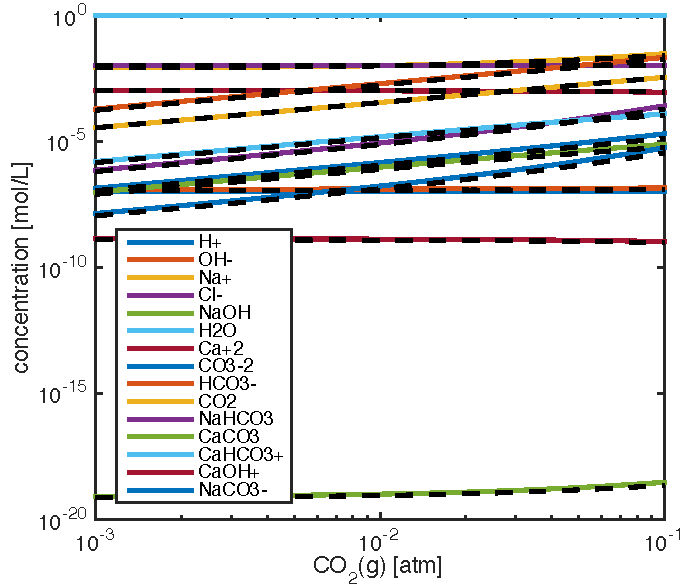
\includegraphics[width=0.9\linewidth]{phases_spec.pdf}
        \caption{aqueous speciation}
    \end{subfigure}%
    ~ 
    \begin{subfigure}[t]{0.5\linewidth}
        \centering
        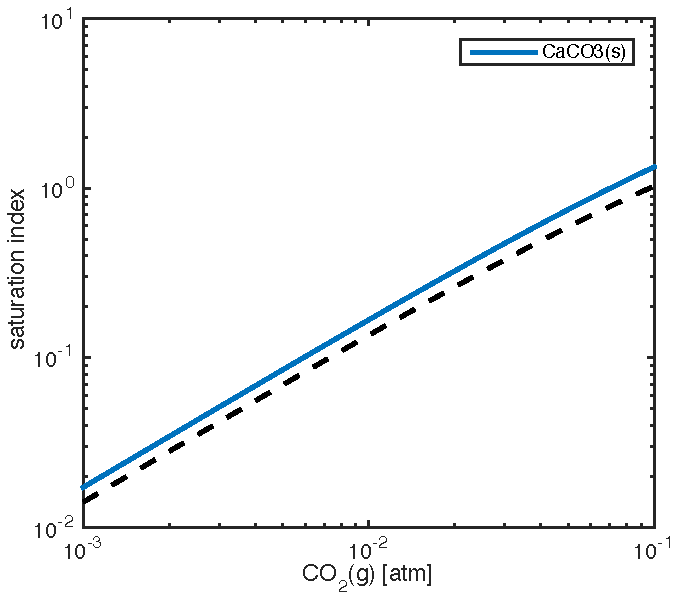
\includegraphics[width=0.9\textwidth]{phases_si.pdf}
        \caption{saturation index}
    \end{subfigure}
    \caption{Comparison of MATCH and PHREEQC for the phases test case for a) aqueous speciation and b) saturation indices. Dashed lines are the results of the PHREEQC simulation.}
    \label{fig:phases}
\end{figure}
It seems the disagreement in the saturation index is likely due to the activity of non-charged species which are calculated by the WATEQ Debye-H\"{u}ckel equation in PHREEQC, and are ignored in MATCH.

\subsection{Surface chemistry}

\subsubsection{Langmuir model}
Here we explore the chemical system

\begin{align}
    \ce{H2O} &= \ce{H+} + \ce{OH-}\\
    \ce{NaOH}&= \ce{Na+} + \ce{OH-}\\
    \ce{SiOH} &= \ce{H+} + \ce{SiO-}\\
    \ce{SiOH} + \ce{H+} &= \ce{SiOH2+}
\end{align}
including charge balance. We explore the effect of pH on surface and aqueous speciation by specifying the inputs

\begin{align}
\Sigma \ce{Na} &= 1\times10^{-2} \quad\text{M}\\
\Sigma \ce{Cl} &= 1\times10^{-2} \quad\text{M}\\
\Sigma \ce{SiO} &= 1.66\times10^{-6} \quad\text{M}\\
[\ce{H+}] &= \texttt{logspace(-3, -11, 100)} \quad\text{M}\\
[\ce{H2O}] & = 1 \quad\text{M}
\end{align}
The MATCH script is

\begin{lstlisting}
elements = {'O', 'H', 'Na*', 'Cl*'};

species = {'H+*', 'OH-', 'H2O*', '>SiO-', '>SiOH', '>SiOH2+', 'Na+', 'Cl-','NaOH'};

reactions = {'H2O  = H+  + OH- ',           10^-14*mol/litre, ...
             '>SiOH = >SiO- + H+',          10^-7.5*mol/litre,...
             '>SiOH + H+ = >SiOH2+',         10^3/(mol/litre),...
             'NaOH = Na+ + OH-',            10^10*mol/litre};

surfInfo = {'>SiO', {[1*site/(nano*meter)^2 1*meter^2/gram 1*gram/litre], 'langmuir'}};

chem = ChemicalModel(elements, species, reactions, 'surfaces', surfInfo);


n = 100;

H2O = ones(n,1);
H   = logspace(-3, -11,n)';
Na  = 1e-2*ones(n,1);
Cl  = Na;

inputs = [Na, Cl, H, H2O]*mol/litre;

[state, report, chem] = chem.initState(inputs, 'chargeBalance', 'Na');
\end{lstlisting}
and the PHREEQC input file is

\begin{Verbatim}[frame=single,fontsize=\footnotesize]
SURFACE_MASTER_SPECIES
	Surf_s	Surf_sOH
SURFACE_SPECIES
     Surf_sOH = Surf_sOH
     log_k = 0
     Surf_sOH = Surf_sO- + H+
     log_k  -7.5
     Surf_sOH + H+= Surf_sOH2+
     log_k  3
SURFACE 1
     Surf_sOH        1    1    1
	-sites_units		density
	-no_edl
END
PHASES
	Fix_H+
		H+ = H+
		log_k  0.0
END
SOLUTION 1
	-units	mol/l
	pH		3
	Na 		1e-2 charge
	Cl 		1e-2
SELECTED_OUTPUT
    -file langmuirTest.out
    -reset false
USER_PUNCH
	10 FOR i = 3 to 11 STEP 0.1
  	20 a$ = EOL$ + "USE SOLUTION 1" + CHR$(59) + " USE SURFACE 1" + EOL$
	30 a$ = a$ + "EQUILIBRIUM_PHASES 1" + EOL$
	40 a$ = a$ + "   Fix_H+ " + STR$(-i) + " NaOH" + EOL$
	50 a$ = a$ + "END" + EOL$
	60 PUNCH a$
	70 NEXT i
END
#
SELECTED_OUTPUT
	-file langmuirTest.sel
	-high_precision true
	-user_punch true
	-molalities H+ OH- Surf_sO- Surf_sOH Surf_sOH2+ Na+ Cl- NaOH
	-ph
USER_PUNCH
INCLUDE$ langmuirTest.out
END
\end{Verbatim}
The results aqueous and surface speciation are plotted in Figure \ref{fig:langmuir}
\begin{figure}[H]
    \centering
    \includegraphics[width=0.7\textwidth]{langmuirTest.pdf}
    \caption{Comparison of MATCH and PHREEQC for the Langmuir test case. Dashed lines are the results of the PHREEQC simulation.}
    \label{fig:langmuir}
\end{figure}

\subsubsection{Ion exchange model}
Here we explore the chemical system

\begin{align}
    \ce{H2O} &= \ce{H+} + \ce{OH-}\\
    \ce{YH} + \ce{Na+} &=  \ce{YNa} + \ce{H+}\\
    \ce{NaOH} &= \ce{Na+} + \ce{OH-}\\
\end{align}
including charge balance, where Y is an exchange site. We explore the effect of pH on the surface and aqueous speciation by specifying inputs as

\begin{align}
\Sigma \ce{Na} &= 1\times10^{-2} \quad\text{M}\\
\Sigma \ce{Cl} &= 1\times10^{-2} \quad\text{M}\\
\Sigma \ce{Y} &= 1.66\times10^{-4} \quad\text{M}\\
[\ce{H+}] &= \texttt{logspace(-3, -11, 100)} \quad\text{M}\\
[\ce{H2O}] & = 1 \quad\text{M}
\end{align}
The MATCH script is

\begin{lstlisting}
elements = {'O', 'H', 'Na*', 'Cl*'};

species = {'H+*', 'OH-', 'H2O*', '>YH', '>YNa', 'Na+', 'Cl-','NaOH'};

reactions = {'H2O  = H+  + OH- ',           10^-14*mol/litre, ...
             '>YH + Na+ = >YNa + H+',       10^-1,...
             'NaOH = Na+ + OH-',            10^10*mol/litre};

surfInfo = {'>Y', {[1*site/(nano*meter)^2 100*meter^2/gram 1*gram/litre], 'ie'}};

chem = ChemicalModel(elements, species, reactions, 'surfaces', surfInfo);

n = 100;

H2O = ones(n,1);
H   = logspace(-3, -11,n)';
Na  = 1e-2*ones(n,1);
Cl  = Na;

inputs = [Na, Cl, H, H2O]*mol/litre;

[state, report, chem] = chem.initState(inputs, 'chargeBalance', 'Na');
\end{lstlisting}
and the PHREEQC input file is

\begin{Verbatim}[frame=single,fontsize=\footnotesize]
EXCHANGE_MASTER_SPECIES
	Y	Y-
EXCHANGE_SPECIES
	Y- = Y-
	-log_k	0
	Na+ + Y- = YNa
	-log_k	0
	 H+ + Y- = YH
	-log_k	1
PHASES
	Fix_H+
		H+ = H+
		log_k  0.0
END
EXCHANGE 1
     Y 1.666e-4
END
SOLUTION 1
	-units	mol/l
	pH		3
	Na 		1e-2 charge
	Cl 		1e-2
SELECTED_OUTPUT
    -file exchangeTest.out
    -reset false
USER_PUNCH
	10 FOR i = 3 to 11 STEP 0.1
  	20 a$ = EOL$ + "USE SOLUTION 1" + CHR$(59) + " USE EXCHANGE 1" + EOL$
	30 a$ = a$ + "EQUILIBRIUM_PHASES 1" + EOL$
	40 a$ = a$ + "   Fix_H+ " + STR$(-i) + " NaOH" + EOL$
	50 a$ = a$ + "END" + EOL$
	60 PUNCH a$
	70 NEXT i
END
#
SELECTED_OUTPUT
	-file exchangeTest.sel
	-high_precision true
	-user_punch true
	-molalities H+ OH- YH YNa Na+ Cl- NaOH
	-ph
USER_PUNCH
INCLUDE$ exchangeTest.out
END

END
\end{Verbatim}
The speciation results are plotted in Figure \ref{fig:exchange}

\begin{figure}[H]
    \centering
    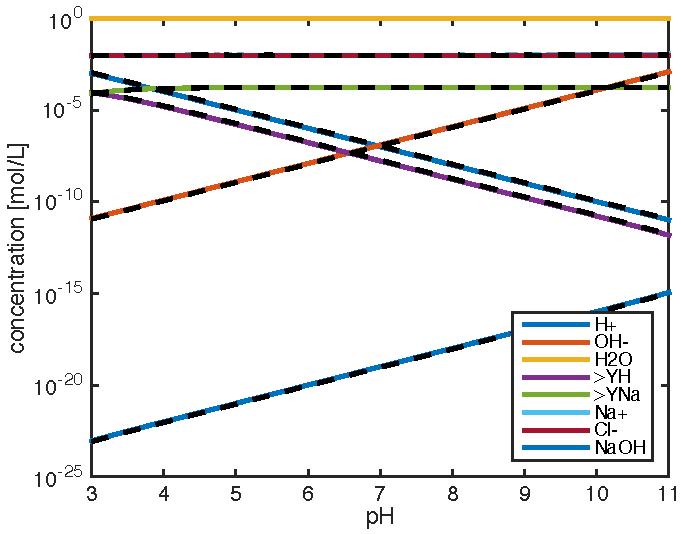
\includegraphics[width=0.7\textwidth]{exchange.pdf}
    \caption{Comparison of MATCH and PHREEQC for the ion exchange test case. Dashed lines are the results of the PHREEQC simulation.}
    \label{fig:exchange}
\end{figure}

\subsubsection{Triple layer model}
Here we explore the chemical system

\begin{align}
    \ce{H2O} &= \ce{H+} + \ce{OH-}\\
    \ce{NaOH}&= \ce{Na+} + \ce{OH-}\\
    \ce{SiOH} &= \ce{H+} + \ce{SiO-}\\
    \ce{SiOH} + \ce{H+} &= \ce{SiOH2+}\\
    \ce{SiO-} + \ce{Na+} &= \ce{SiONa}\\
    \ce{SiOH2+} + \ce{Cl-} &= \ce{SiOH2Cl}
\end{align}
including charge balance. We explore the effect of pH on the surface and aqueous speciation by specifying inputs as

\begin{align}
\Sigma \ce{Na} &= 1\times10^{-2} \quad\text{M}\\
\Sigma \ce{Cl} &= 1\times10^{-2} \quad\text{M}\\
\Sigma \ce{SiO} &= 1.66\times10^{-6} \quad\text{M}\\
[\ce{H+}] &= \texttt{logspace(-3, -11, 100)} \quad\text{M}\\
[\ce{H2O}] & = 1 \quad\text{M}
\end{align}

The MATCH script is

\begin{lstlisting}
elements = {'O', 'H', 'Na*', 'Cl*'};

species = {'H+*', 'OH-', 'Na+', 'Cl-', 'NaOH', 'H2O*',...
             '>SiO-', '>SiOH', '>SiOH2+', '>SiONa', '>SiOH2Cl'};

reactions ={'H2O  = H+  + OH- ',          10^-14*mol/litre, ...
            'NaOH = Na+ + OH-',           10^10*mol/litre,...
            '>SiOH = >SiO- + H+',           10^-7.5*mol/litre,...
            '>SiOH + H+ = >SiOH2+',         10^3/(mol/litre),...
            '>SiO- + Na+ = >SiONa',         10^-2/(mol/litre),...
            '>SiOH2+ + Cl- = >SiOH2Cl',     10^-2/(mol/litre)};
        
geometry = [1*site/(nano*meter)^2 1*meter^2/gram 1*gram/litre];
sioInfo = {geometry, 'tlm', [1 0.2],	'>SiONa',   [-1 1], '>SiOH2Cl',[1 -1]};
surfaces ={ '>SiO', sioInfo };

chem = ChemicalModel(elements, species, reactions, 'surf', surfaces);

chem.printChemicalSystem;

n = 100;

Na = 1e-2*ones(n,1);
Cl = 1e-2*ones(n,1);
H = logspace(-3, -11, n)';
H2O = ones(n,1);

state = chem.initState([Na Cl H H2O]*mol/litre, 'chargeBalance', 'Na');
\end{lstlisting}
and the PHREEQC input file is

\begin{Verbatim}[frame=single,fontsize=\footnotesize]
SURFACE_MASTER_SPECIES
	Surf_s	Surf_sOH
SURFACE_SPECIES
     Surf_sOH = Surf_sOH
     log_k = 0
     Surf_sOH = Surf_sO- + H+
     log_k  -7.5
	-cd_music -1 0 0
     Surf_sOH + H+= Surf_sOH2+
     log_k  3
	-cd_music 1 0 0
     Surf_sO- + Na+ = Surf_sONa
     log_k  -2
	-cd_music 0 1 0
     Surf_sOH2+ + Cl- = Surf_sOH2Cl
     log_k  -2
	-cd_music 0 -1 0
SURFACE 1
     Surf_sOH        1    1    1
	-sites_units		density
	-cd_music
	-capacitances		1	0.2
END
PHASES
	Fix_H+
		H+ = H+
		log_k  0.0
END
SOLUTION 1
	-units	mol/l
	pH		3
	Na 		1e-2 charge
	Cl 		1e-2
SELECTED_OUTPUT
    -file tripleLayerTest.out
    -reset false
USER_PUNCH
	10 FOR i = 3 to 11 STEP 0.1
  	20 a$ = EOL$ + "USE SOLUTION 1" + CHR$(59) + " USE SURFACE 1" + EOL$
	30 a$ = a$ + "EQUILIBRIUM_PHASES 1" + EOL$
	40 a$ = a$ + "   Fix_H+ " + STR$(-i) + " NaOH" + EOL$
	50 a$ = a$ + "END" + EOL$
	60 PUNCH a$
	70 NEXT i
END
#
SELECTED_OUTPUT
	-file tripleLayerTest.sel
	-high_precision true
	-user_punch true
	-molalities H+ OH- Surf_sO- Surf_sOH Surf_sOH2+ Surf_sONa Surf_sOH2Cl Na+ Cl- NaOH
	-ph
USER_PUNCH
INCLUDE$ tripleLayerTest.out
END
\end{Verbatim}
The aqueous speciation results are plotted in Figure \ref{fig:triple}
\begin{figure}[H]
    \centering
    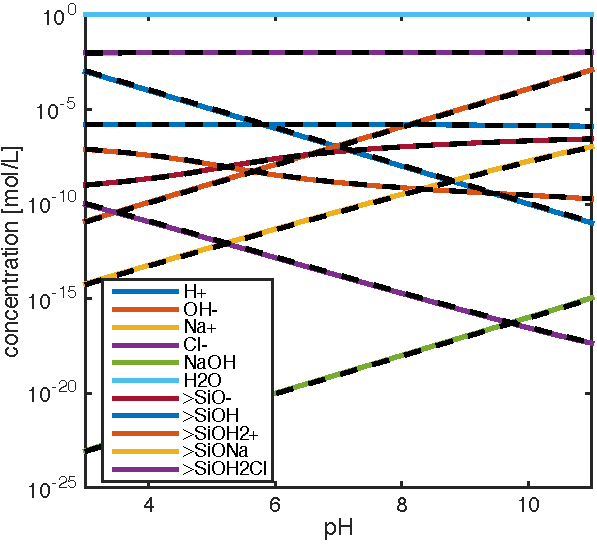
\includegraphics[width=0.7\textwidth]{tripleLayerTest.pdf}
    \caption{Comparison of MATCH and PHREEQC for the triple layer model test case. Dashed lines are the results of the PHREEQC simulation.}
    \label{fig:triple}
\end{figure}

\bibliographystyle{plainnat}
\bibliography{references}
\end{document}
